\documentclass[a4paper,12pt]{article}
\usepackage{amsfonts}
\usepackage{amsmath}
\usepackage{graphicx}
\usepackage{amssymb}
\usepackage{array}
\usepackage[round]{natbib}
\usepackage{booktabs}
\usepackage{floatpag}
\usepackage[hmargin=2.5cm,vmargin=3cm]{geometry}
\usepackage{setspace}
\usepackage{chngcntr}
\usepackage{verbatim}
\usepackage{multirow}
\usepackage{url}
\usepackage{doi}
\usepackage{hyperref}
\usepackage{xcolor}
\hypersetup{
    colorlinks,
    linkcolor={blue!50!black},
    citecolor={blue!50!black},
    urlcolor={blue!80!black}
}

\usepackage[gen]{eurosym}
\floatpagestyle{plain}
\newcolumntype{H}{>{\setbox0=\hbox\bgroup}c<{\egroup}@{}}
\renewcommand{\floatpagefraction}{0.95}
\setstretch{1.5}
\newcommand{\pathTables}{../workm_lp/}
\newcommand{\pathFigures}{}
\newcommand{\pathA}{}
\newcommand{\pathB}{}
\newcommand{\pathC}{}
\begin{document}
\pagenumbering{gobble}

\author{Marek Jaroci\'nski\thanks{%
European Central Bank DG-Research, email: marek.jarocinski@ecb.europa.eu}}
\title{Central Bank Information Effects and Transatlantic Spillovers\thanks{%
The opinions in this paper are
those of the author and do not necessarily reflect the views of the
European Central Bank.
This is a revised version of the paper ``International spillovers of the Fed and ECB monetary policy surprises'', 2018. I thank Luca Dedola, Pierre De Leo, Wouter den Haan, Georgios Georgiadis, Refet G\"urkaynak, Marcin Kasperczyk, Arvind Krishnamurthy, Friederike Niepmann, Giorgio Primiceri, John Rogers, Georg Strasser, seminar and conference participants, anonymous referees and the associate editor for their comments. I thank Jonas Jensen for help with accessing high frequency data and sharing his expertise in this field. Anke Witteler provided outstanding research assistance.}}
\date{\today}
\maketitle

\begin{abstract}
News about the economy contained in a central bank announcement can affect public expectations. This paper shows, using both event studies and vector autoregressions, that such central bank information effects are an important channel of the transatlantic spillover of monetary policy. They account for a part of the co-movement of German and US government bond yields around Fed policy announcements,
and for most of this co-movement around ECB policy announcements.
Consequently, ECB surprise interest rate hikes that spill over to US government bond yields are followed on average by easier, not tighter, US financial conditions and an economic expansion.
In fact, they spill over similarly as positive European macroeconomic news surprises.
By contrast, pure ECB ``monetary policy shocks'' do not spill over,
in part because of the offsetting Fed policy stance.


\bigskip

\noindent \textbf{JEL Classification}: E52, F31, F42

\noindent \textbf{Keywords}: International Policy Transmission, Monetary Policy Shocks, High-Frequency Identification, Structural VAR
\end{abstract}


\pagebreak

\setcounter{page}{1}\pagenumbering{arabic}

\section{Introduction}

The yields on the US and German government bonds often co-move on the days when the Fed or the ECB announce their policy decisions.
This is one manifestation of the transatlantic spillovers of monetary policies through integrated financial markets.
A large literature documents that when the Fed hikes its interest rate, financial conditions tighten and the economic activity declines also outside of the US borders \citep[][and many others]{Rey_2013,MirandaAgrippino_Rey_2020}. 
But, as repeatedly pointed out by the Fed officials, the Fed is not the only central bank whose actions affect global financial markets \citep[e.g.][]{Powell_2018,Clarida_2021}.
US and European government bond yields co-move also around ECB policy announcements \citep[e.g.][]{Curcuru_etal_2018}.
However, the empirical evidence on the effects of ECB policies on the US is often counter-intuitive and the published literature on it is scarce.

This paper dissects an empirical puzzle that has plagued this research. It
shows that an ECB interest rate hike that spills over across the Atlantic is followed
by an easing, not a tightening, of the US financial conditions and an expansion of economic activity.
This paper argues that the evidence is consistent with a weak transatlantic spillover of the ECB monetary policies and
a strong transatlantic spillover of the ECB information effects. 
The latter mean that investors facing a positive interest rate
surprise infer that the ECB is more bullish about the economy than they expected and this makes them more bullish as well \citep{Romer_Romer_2000,Nakamura_Steinsson_2018}.
 In fact, as this paper shows, when the US financial variables respond to ECB interest rate hikes,
their response is similar to their response to unexpectedly positive euro area macroeconomic data releases.

I first document that the transatlantic spillovers of ECB interest rate surprises are conditional
on the co-movement of European interest rates and stock prices.
Not all ECB interest rate surprises generate a persistent, same-sign effect on the US Treasury yields.
It is only those that are associated with a positive co-movement of European interest rates and stock prices.
Hence, these transatlantic spillovers cannot be driven by ECB monetary policy shocks,
which would have driven these two variables in the opposite directions.
I construct proxies for ECB monetary policy and information shocks based on the
high-frequency co-movement of interest rates and stock prices in the wake of policy announcements, following \cite{Jarocinski_Karadi_2020}.
It is the ECB information shocks that spill over to the Treasury yields.

Next, I study the responses of other US variables to ECB shocks
using daily event study regressions and monthly vector autoregressions (VARs).
The ECB information shocks significantly affect a range of US financial variables, 
including stock prices, corporate bond spreads and the dollar exchange rate, also against currencies
other than the euro, and are eventually followed by stronger US real activity and higher prices.

For a comparison, I estimate the transatlantic spillovers of selected European macroeconomic news surprises,
defined as the differences between the actual data releases and their earlier expectations from Bloomberg surveys of professional forecasters.
I find that the US financial markets respond to an ECB information shock similarly as they do
to an unexpectedly high reading of the European industrial confidence or an unexpectedly low European unemployment rate.

I show that the responses of the US stock prices are not driven by companies doing business with Europe.
Predominantly US-exposed companies respond no less. The stocks that respond the most to ECB information shocks are those that are particularly sensitive to general investor sentiment: financial stocks and small stocks \citep{Baker_Wurgler_2006}.

Finally, using the same methodology and variables I study the effects of the Fed shocks on the euro area. I find similar transatlantic spillovers of the Fed information shocks in the monthly VAR.
In the case of the Fed I also find strong spillovers of the monetary policy shock, consistently with the consensus in the literature.

These results reconcile two facts. On the one hand, research finds that the transatlantic financial spillovers work both ways, also from Europe to the US. The already mentioned paper by 
\cite{Curcuru_etal_2018} documents a positive co-movement of long-term US Treasury and German bund yields on the days of ECB policy announcements. 
For another example, \cite{Ehrmann_etal_2011} find significant spillovers of European shocks to the US across several asset classes.
On the other hand, there is a dearth of published evidence on the effects of ECB policy on the US risky asset prices and financial conditions, while
some papers note in passing that these effects appear puzzling \citep[e.g.][]{Rogers_Scotti_Wright_2014,Brusa_etal_2020}.
Most of the literature on the international spillovers of ECB monetary policies focuses on the non-eurozone European countries \citep[e.g.][]{Bluwstein_Canova_2016,Moder_2019,Feldkircher_etal_2020,terEllen_etal_2020,Corsetti_etal_2021},
on specific subsets of monetary policy interventions \citep{Georgiadis_Grab_2016}, or both.

This paper shows that it is exactly those ECB surprises that generate information effects at home,
according to the \cite{Jarocinski_Karadi_2020} decomposition, that are responsible for the bulk of the transatlantic spillovers.
Hence, the response of US financial variables to these ECB surprises is not puzzling.
It is similar to the effect of other European macroeconomic news.

What is more puzzling is the weak spillover of the ECB monetary policy to the US.
This weak spillover is likely to result from a combination of two factors.
First, the ECB monetary policy shocks have a smaller direct effect
on the US economy than the other European shocks.
Second, the Fed offsets the ECB monetary policy shocks more effectively.
The first observation is intuitive, if we think of the other European shocks as containing a combination of a purely European shock (say, a wage bargaining round by trade unions in France) and a global shock (say, a global commodity supply shock). Such a combined shock will affect both those US companies that do business with Europe and those that do not. By contrast, an ECB monetary policy shocks affects directly only the US companies that do business with Europe.
This intuition is consistent with this paper's findings on the responses of Europe-exposed vs US-exposed US stocks.
The second observation is intuitive if we consider that the ECB monetary policy 
shock is a shock to financial conditions and the Fed
is particularly well equipped to offset its effect on the US financial conditions, given that
the role of the dollar as an investing and funding currency dwarfs that of the euro \citep{Rey_2016}.
In fact, this is what the Fed seems to be doing: indicators of Fed policy stance, such as the effective fed funds rates, shadow fed funds rates and US Treasury yields, fall in response to contractionary ECB monetary policy shocks.

The aforementioned large literature that documents strong international spillovers of the Fed's monetary policy includes also \cite{Kim_2001,Mackowiak_2007,Georgiadis_2016,Ha_2016, Dedola_Rivolta_Stracca_2017,Gerko_Rey_2017,Degasperi_etal_2021} and many others.
The literature on central bank information effects goes back to \cite{Romer_Romer_2000}.
\cite{Melosi_2017,Nakamura_Steinsson_2018} build theoretical models featuring these effects and
\cite{Campbell_etal_2012,Cieslak_Schrimpf_2019,Jarocinski_Karadi_2020,Andrade_Ferroni_2021,MirandaAgrippino_Ricco_2021}, among others,
provide empirical evidence. \cite{Kroencke_etal_2021} document a related phenomenon of the ``FOMC risk shift.'' The Neo-Fisher effect, studied by \cite{Uribe_2022} and others, is an alternative mechanism that leads to expansionary interest rate hikes.
Also \cite{Bauer_Swanson_2020} and \cite{Sastry_2021} propose alternative explanations of the central bank information effects. 

This paper belongs to the growing recent literature on the contribution of central bank information effects to international spillovers. 
\cite{CesaBianchi_Sokol_2022} document the spillovers of Fed information shocks to Europe.
\cite{Hoek_etal_2022} report differential responses of emerging markets to Fed monetary and information shocks.
In \cite{Stavrakeva_Tang_2021} and \cite{Gurkaynak_etal_2021} central bank information effects help explain the behavior of the exchange rate. \cite{Bekaert_Hoerova_Xu_2020} find strong non-
monetary policy-driven risk and uncertainty spillovers across countries, emanating not just from the US but also from the euro area and Japan. In particular, independently from this paper they confirm the significant spillovers of ECB information effects to the US financial variables. 
\cite{Franz_2020} studies a panel of exchange rates and shows that speculative currencies appreciate after positive ECB information shocks. Furthermore, controlling for central bank information effects is important for precisely isolating the spillovers of monetary policy shocks in \cite{Cazorzi_etal_2020,MirandaAgrippino_Rey_2020,Corsetti_etal_2021,MirandaAgrippino_Nenova_2021}.

The rest of the paper is organized as follows. Section 2 explains the identification of shocks.
Section 3 documents the conditional transatlantic spillovers of the ECB interest rate surprises to US Treasury yields.
Section 4 reports the responses of other US variables.
Section 5 compares the spillovers of ECB surprises with those of other European macroeconomic news.
Section 6 focuses on the responses of the Fed policy stance to ECB monetary policy shocks.
Section 7 reports the transatlantic spillovers of the Fed shocks.
Section 8 concludes.

\section{Central bank interest rate surprises and their two components}\label{sec: surprises}

Monetary policy reacts to the state of the economy, reflecting a variety of global and
domestic shocks. In order to isolate the international spillovers of central bank policies
from the international spillovers of other shocks, this paper focuses on central bank interest rate \emph{surprises}. 
These are defined as the high-frequency reactions of market interest rates to central bank announcements.
Furthermore, I decompose the interest rate surprises into two distinct components.

\subsection{Central bank surprises}

When a central bank begins to announce its policy, markets have already priced in its systematic response
to the state of the economy. 
Therefore, the surprise is exogenous to this systematic response and, hence, useful for isolating the causal effects of the central bank communication and action.
The use of surprises for identification goes back at least to \cite{Kuttner_2001}. I
take the ECB surprises from the dataset of \cite{Altavilla_etal_2019}
and the Fed surprises from the dataset of \cite{Gurkaynak_Sack_Swanson_2005a} updated by \cite{Gurkaynak_Karasoy_Lee_2022} and
complemented to include also the effect of the Fed press conferences (as in the \citealt{Altavilla_etal_2019} dataset).
Since the focus of this paper is on the transatlantic spillovers, I drop simultaneous policy announcements
by the Fed and the ECB.

The Euro Area Monetary Policy Event-Study Database (EA-MPD) of \cite{Altavilla_etal_2019}
includes all the monetary policy announcements that follow ECB Governing Council meetings.
I use the surprises in the ``Monetary Event'' window: a half-hour window around the press release, extended until 15 minutes after the end of the press conference whenever there is one.
The EA-MPD vintage used in this paper contains 264 announcements from 7 January 1999 to 6 June 2019. I drop three coordinated, same-day policy announcements by the Fed and the ECB: on 13 and 17 September 2001 and on 8 October 2008. This leaves 261 ECB announcements.

The Fed surprises are based on the \cite{Gurkaynak_Sack_Swanson_2005a} (GSS) database
updated until June 2019 by \cite{Gurkaynak_Karasoy_Lee_2022}
and adjusted to reflect also the Fed press conferences.
The GSS data contain the surprises in a half-hour window around the press releases.
Therefore, on the days when a press conference was also held I take the sum of the GSS surprise and the surprise in the press conference window.
I use Thomson Reuters Tick History database to measure
the surprises in the press conference window. 
The press conference window starts (in most cases) at the end of the GSS window and 
ends 15 minutes after the end of the press conference,
resulting in a similar ``Monetary Event'' window as for the ECB.
See Appendix \ref{sec: Fed press conf} for further details on the financial market surprises during the Fed press conferences.
For comparability with the ECB I start the sample in 1999 and end in June 2019. I drop three coordinated, same-day policy announcements by the Fed and the ECB: on 17 September 2001, 11 March 2008 and 8 October 2008 (the second one is not present in the EA-MPD). This leaves 171 announcements

For each dataset I compute the summary \textbf{interest rate surprise}, $i^{Total}$ and \textbf{stock price surprise}, $s$.
The interest rate surprise is the first principal component of the surprises in interest rate derivatives with maturities up to 1 year. 
For the Fed, following e.g. \cite{Gurkaynak_Sack_Swanson_2005a} and \cite{Nakamura_Steinsson_2018}, I use the current month and 3-month fed funds futures and 2-, 3-, and 4- quarters ahead 3-month eurodollar futures.
For the ECB I use the Overnight Index Swaps (OIS) with maturities 1-, 3- and 6-months and 1-year.\footnote{The choice of instruments is motivated by their liquidity. The OIS swaps are the most liquid instruments in Europe while the eurodollar futures are the most liquid instruments in the US. When comparing the two surpries, the caveat is that the eurodollar rates include a slightly larger credit risk component than the Eonia rate underlying the OIS swaps.}
I rescale each interest rate surprise so that they have the standard deviations of the respective 1-year instruments (fourth eurodollar future and 1-year OIS swap respectively).
For the Fed stock price surprises I use the S\&P500 index and for the ECB stock price surprises I use the Euro Stoxx 50 index.


\subsection{Decomposing interest rate surprises into monetary policy and information shocks}

Next, I follow  \cite{Jarocinski_Karadi_2020} and decompose the total interest rate surprises
based on their correlation with the stock price surprises, as
\begin{equation}
i^{Total} = i^{MP}+i^{CBI}.\label{eq: decomposition}
\end{equation}
where $i^{MP}$ is negatively correlated with $s$ and $i^{CBI}$ is positively correlated with $s$.

According to a textbook asset pricing model, monetary policy shocks generate a negative correlation between the interest rate and stock price surprises. For example, an expansionary monetary policy shock reduces the discount rate and increases the expected future dividends, so the stock price, which reflects the present discounted value of future dividends, increases. This justifies thinking of $i^{MP}$ as a proxy for a Monetary Policy (MP) shock.

Since the $i^{CBI}$ component is positively correlated with $s$, it follows that it is not a monetary policy shock.
\cite{Jarocinski_Karadi_2020} propose to treat it as a proxy for the Central Bank Information (CBI) effect.
If the state of the economy is imperfectly observable, agents facing a positive interest rate surprise
infer that the central bank is more bullish about the economy than they expected 
and this makes them more bullish as well.\footnote{See e.g. \cite{Romer_Romer_2000,Melosi_2017,Nakamura_Steinsson_2018}.
The central bank does not need to have superior knowledge about the economy to affect
agents' expectations, it is enough if its forecast is not perfectly correlated with agents' forecasts. In fact, \cite{Morris_Shin_2002} show that, in the presence of coordination motives,
the central bank's public forecast can have outsized effects even if it is less precise than the agents' private forecasts.}
The precise origins of these surprises continue to be debated.
The Neo-Fisher effect is another mechanism that can generate a positive correlation
between interest rate surprises and stock price surprises.
E.g. \cite{Uribe_2022} argues that when an interest rate increase is perceived to be permanent,
inflation expectations rise sufficiently fast to temporarily depress the real interest rate,
stimulating output. In another vein, \cite{Bauer_Swanson_2020} propose
a ``Fed response to economic news'' effect to explain the positive correlation between interest rate surprises and subsequent revisions of survey expectations. 
To the extent that the ``Fed response to economic news'' can also generate
a positive correlation between interest rate surprises and stock price surprises, 
one can interpret the $i^{CBI}$ as a proxy for this effect too.
The bottom line is that the impact of a positive $i^{CBI}$ (unlike $i^{MP}$) is similar to the impact of \emph{positive} economic news.

More in detail, I compute a decomposition that satisfies
\begin{equation}\label{eq: rotational}
M = UC,\;\;\text{with}\;\;  U'U=\text{diagonal matrix} \;\; \text{and}\;\;
C=\begin{pmatrix}1&c_{MP}<0\\1&c_{CBI}>0\end{pmatrix},
\end{equation}
where $M=(i^{Total},s)$ is a $T \times 2$ matrix with $i^{Total}$ in the first column and $s$ in the second column,
$U=\left(i^{MP},i^{CBI}\right)$ is a $T \times 2$ matrix with $i^{MP}$ in the first column and $i^{CBI}$ in the second column, $T$ is the number of central bank announcements,
$i^{MP}$ and $i^{CBI}$ are mutually orthogonal, and matrix $C$ captures how $i^{MP}$ and $i^{CBI}$ translate
into financial market surprises. The 1's in the first column of $C$ reflect equation (\ref{eq: decomposition}).
The second column of $C$ contains the elasticities of stock prices to $i^{MP}$ and $i^{CBI}$, $c_{MP}<0$ and $c_{CBI}>0$.

\newcommand{\vsmp}{\frac{\operatorname{var}(i^{MP})}{\operatorname{var}(i^{Total})}}
\newcommand{\vscbi}{\frac{\operatorname{var}(i^{CBI})}{\operatorname{var}(i^{Total})}}

The decomposition in (\ref{eq: rotational}) is not unique. 
If we ``rotate'' $U$ and $C$ with an orthogonal matrix, the new shocks $\tilde{U}$ will still be
orthogonal and for many rotation angles
the sign restrictions $c_{MP}<0$ and $c_{CBI}>0$ will still be satisfied.
Smaller rotation angles yield decompositions with less negative $c_{MP}$ and larger $c_{CBI}$,
so monetary policy shocks 
account for more variation of the interest rates and central bank information accounts for more variation of the stock prices.
Larger rotation angles yield decompositions with more negative $c_{MP}$ and smaller $c_{CBI}$,
so monetary policy shocks 
account for more variation of the stock prices and central bank information accounts for more variation of the interest rates.
To obtain a point estimate I follow \cite{Fry_Pagan_2011} and compute the Median Target rotation, which here boils down to using the median of the admissible rotation angles.
For the Fed this yields the coefficients $c_{MP}=-9.9$ and $c_{CBI}=9.9$.
(At the median rotation the coefficients have the same absolute value.)
\citet[][section VI.B]{Nakamura_Steinsson_2018} find similar numbers using their structural model:
$c_{MP}=-11.1$ with the 95\% confidence interval [-19.4, -2.5]. 
The coefficients for the ECB are $c_{MP}=-c_{CBI}=-15.7$.
In robustness exercises I first report the decompositions corresponding to a few other rotation angles and then randomize over all rotations consistent with the sign restrictions.
This last approach reflects an agnostic prior about the rotation.

Figure \ref{fig: cumulated shocks} plots the cumulated shocks obtained with the median rotation.
The Online Appendix provides the details on the computation of the decomposition.


\begin{figure}[!htbp]
\caption{Cumulated shocks}\label{fig: cumulated shocks}
\begin{center}
\begin{tabular}{cc}
\small $i^{MP}$ & \small $i^{CBI}$ \\
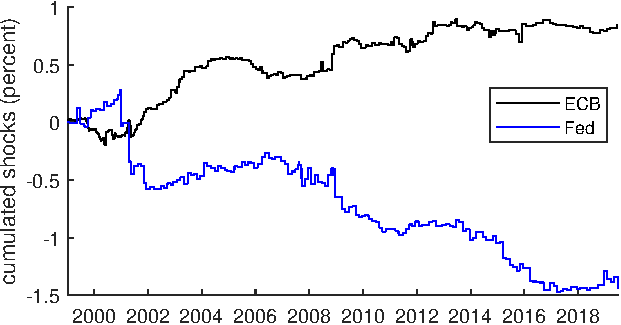
\includegraphics[width=0.47\textwidth]{figures/cumulated_mp_median} &
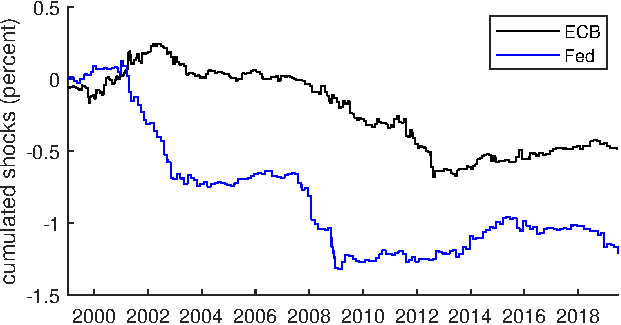
\includegraphics[width=0.47\textwidth]{figures/cumulated_cbi_median}\\
\end{tabular}
\end{center}
\end{figure}

As another robustness check, I also perform a simple decomposition, dubbed ``poor man's sign restrictions'' in \cite{Jarocinski_Karadi_2020}, where
I simply classify each central bank announcement as conveying either $i^{MP}$ or $i^{CBI}$.
\begin{equation}
i^{MP} = \begin{cases} i^{Total} &\text{if} \quad  i^{Total}\times s\le0\\ 0 &\text{otherwise}\end{cases},\qquad
i^{CBI} = \begin{cases} 0 &\text{if} \quad  i^{Total}\times s\le0\\ i^{Total} &\text{otherwise.}\end{cases}
\end{equation}
This simple approach is more restrictive because it assumes that only one type of shock, either
MP or CBI, is present in a given announcement. The rotation-based decomposition
allows both shocks to be present in the same announcement.

\section{Conditional transatlantic spillover of ECB interest rate surprises}

This section documents a new stylized fact about the transatlantic spillovers of ECB interest rate
surprises: they are conditional on the direction of the response of the European stock prices.
The ECB interest rate surprises spill over to the US Treasury yields
when on impact European interest rates and stock prices co-move positively.
By contrast, there is no detectable transatlantic spillover when on impact
European interest rates and stock prices co-move negatively, i.e. after an ECB monetary policy shock.

To examine the transatlantic spillovers I run the following event study regressions (local projections):
\begin{equation}
y^{}_{t+h}-y^{}_{t-1} = \alpha + \beta^{MP}_h\, i^{MP}_t + \beta^{CBI}_h\, i^{CBI}_t + u_t.\label{eq: event study reg 2}
\end{equation}
$t$ runs over the dates of ECB monetary policy announcements (261 dates in the EA-MPD, from 7 January 1999 to 6 June 2019). $y^{}$ denotes a financial variable of interest, in the baseline case this is the 1-year US Treasury yield. 
$h$ is the horizon, in business days. I run the regressions for $h=1,2,3,4,5,10,15,...$
I include $i^{MP}_t$ and $i^{CBI}_t$ simultaneously as explanatory variables but they are mutually orthogonal so their estimated coefficients would be the same if estimated one by one.
$\beta_h^{MP}$ and $\beta_h^{CBI}$ are the coefficients of interest, showing by how many basis points $y$ changes over $h$ days per one basis point of $i^{MP}_t$ and $i^{CBI}_t$. Throughout the paper I use the Eicker-Huber-White heteroskedasticity-robust standard deviations. In most of the sample ECB announcements are separated by about a month and Fed announcements by about seven weeks, so the horizons rarely overlap, thus obviating the need to use autocorrelation-robust standard deviations.

\begin{table}[!htbp]
\begin{center}
\caption{The effect of ECB monetary policy and information shocks on financial variables}\label{tab: lp ecb shocks 1y}
$y^{}_{t+h}-y^{}_{t-1} = \alpha + \beta^{MP}_h\, i^{MP}_t + \beta^{CBI}_h\, i^{CBI}_t + u_t.$
\small
\resizebox{\textwidth}{!}{
\begin{tabular}{lcccccccHHH} \toprule
 & $h=1$ & $h=2$ & $h=3$ & $h=4$ & $h=5$ & $h=10$ & $h=15$ & $h=20$ & $h=25$ & $h=30$
\input{\pathTables table-ecbshocks1a.txt}
\tabularnewline \bottomrule
\end{tabular}}
\end{center}\footnotesize
Notes: Heteroskedasticity robust standard errors in parentheses. *** p$<$0.01, ** p$<$0.05, * p$<$0.1.
Constant terms are not reported for brevity.
F-test: p-value of the F-test for H0: $\beta^{MP}_h=\beta^{CBI}_h$.
\end{table}

\begin{table}[!htbp]
\begin{center}
\caption{The effect of ECB monetary policy and information shocks on US Treasury yields for other rotations}\label{tab: lp ecb shocks 1y pctiles}
$y^{}_{t+h}-y^{}_{t-1} = \alpha + \beta^{MP}_h\, i^{MP}_t + \beta^{CBI}_h\, i^{CBI}_t + u_t.$
\small
\resizebox{\textwidth}{!}{
\begin{tabular}{lcccccccHHH} \toprule
 & $h=1$ & $h=2$ & $h=3$ & $h=4$ & $h=5$ & $h=10$ & $h=15$ & $h=20$ & $h=25$ & $h=30$
\input{\pathTables table-ecbshocks1b1.txt}\\[-0.5cm]
Share $\beta^{MP}$ significant 
& 0.01 & 0.00 & 0.00 & 0.14 & 0.02 & 0.03 & 0.00 & 0.32 & 0.57 & 0.52 \\
Share $\beta^{CBI}$ significant 
& 0.52 & 0.69 & 0.75 & 0.68 & 0.50 & 0.17 & 0.00 & 0.00 & 0.00 & 0.27 \\
%\input{\pathTables table-ecbshocks1b2.txt}\\[-0.5cm]
%Share $\beta^{MP}$ significant 
%& 0.86 & 0.81 & 0.79 & 0.66 & 0.59 & 0.37 & 0.41 & 0.30 & 0.30 & 0.24 \\
%Share $\beta^{CBI}$ significant 
%& 1.00 & 1.00 & 1.00 & 1.00 & 1.00 & 1.00 & 1.00 & 1.00 & 1.00 & 1.00 \\
\tabularnewline \bottomrule
\end{tabular}}
\end{center}\footnotesize
Notes: Heteroskedasticity robust standard errors in parentheses. *** p$<$0.01, ** p$<$0.05, * p$<$0.1.
Constant terms are not reported for brevity.
F-test: p-value of the F-test for H0: $\beta^{MP}_h=\beta^{CBI}_h$.
Share $\beta^{MP}$ ($\beta^{CBI}$) significant: share of all admissible rotations for which $\beta^{MP}$ ($\beta^{CBI}$) is significant at the 0.1 level.
\end{table}

Table \ref{tab: lp ecb shocks 1y} reveals a striking contrast between the transatlantic spillovers
of the two components of the ECB interest rate surprises.
The interest rate surprises
that on impact move the European stock prices in the same direction ($i^{CBI}$) have a significant effect
on the US Treasury yields. 
For the median rotation-based decomposition the effect of a 1 basis point $i^{CBI}$ on the US 1-year Treasury yield
ranges from 0.29 after one day to 0.48 basis points after three days. 
For the simple decomposition (``poor man's sign restrictions'') the effect ranges from 0.53 after one day to 0.69 after three days.
These are substantial, economically significant spillovers. They are also statistically significant at the 10\% level or higher for the first five days.
By contrast, the impact effects of $i^{MP}$ are very small and statistically insignificant for both decompositions. On the subsequent days the point estimates actually turn negative and get more negative over time (though do not become statistically significant).
Table \ref{tab: lp ecb shocks 1y} reports also the p-values obtained when testing
the null hypothesis that $\beta^{MP}_h=\beta^{CBI}_h$, showing that for many horizons we can
reject this null hypothesis.

These results shed new light on the transatlantic spillovers of ECB interest rate surprises.
We know from the meticulous examination of high-frequency futures prices by \cite{Curcuru_etal_2018} that long-term US and German yields are strongly positively correlated in a narrow time-window around ECB announcements. 
This is commonly seen as evidence that the ECB monetary policies spill over to the US.
This important evidence has featured
in high-level policy statements about international monetary policy spillovers \citep{Powell_2018,Clarida_2021}. 
However, the results in Table \ref{tab: lp ecb shocks 1y} imply that positive monetary policy spillovers
are persistent enough to show up in daily data only when the European interest rates and stock prices co-move positively.
This means that ECB monetary policy shocks cannot be the driver of these spillovers, as monetary
policy would drive the interest rates and stock prices in the opposite directions.

To add more context to these numbers, Table \ref{tab: lp ecb shocks 1y}  reports also the responses of 1-year German bund yields. Unlike the US Treasuries, German bund yields are strongly affected by all ECB surprises,
both $i^{MP}$ and $i^{CBI}$.
The effect of $i^{CBI}$ is stronger and more persistent (similarly as in the VAR results of \citealp{Jarocinski_Karadi_2020}), but the impact effect of $i^{MP}$ is substantial and highly significant too. 

Table \ref{tab: lp ecb shocks 1y pctiles} reports analogous regressions for the decompositions obtained with the 25th and 75th percentile rotations. The 25th percentile decomposition, in which
monetary policy account for more variation of the interest rates and central bank information accounts for more variation of the stock prices, compared with the median,
 yields a very similar finding: significant positive spillovers of the $i^{CBI}$ shocks
and their absence for the $i^{MP}$ shocks. For the 75th percentile decomposition the spillovers
of the $i^{CBI}$ shocks cease to be statistically significant (except for the 3-day horizon)
but their point estimates continue to be positive, while the point estimates of $i^{MP}$
effects turn consistently negative and we continue to reject the null hypothesis that $\beta^{MP}_h=\beta^{CBI}_h$ for most horizons. So, we are not any closer to finding a positive spillover of $i^{MP}$. This holds also for even more extreme rotations.
Table \ref{tab: lp ecb shocks 1y pctiles} reports also the shares of all admissible rotations for which each coefficient is significant at the 0.1 level. For horizons up to 5 days these shares exceed 0.5 for $\beta^{CBI}$. For $\beta^{MP}$ they are negligible and correspond to negative coefficients.
To summarize, across rotations we find that any positive impact of the ECB interest rate surprises on the US Treasury yields is coming from $i^{CBI}$ rather than $i^{MP}$. One can construct decompositions for which the positive spillover of $i^{CBI}$ is statistically insignificant, but for a majority of rotations the positive spillover of $i^{CBI}$ is statistically significant.


The transatlantic spillover of the total interest rate surprise $i^{Total}$ to the US Treasury yields, either at the 1-year or 10-year maturity, is not significant. However, the $i^{CBI}$ component of the total interest rate surprise
i) has a much stronger effect on the 10-year German Bund yield and ii) spills over to the 10-year US Treasury yields. By contrast, the $i^{MP}$ component has a weaker effect on the 10-year German Bund yield and does not spill over to the 10-year US Treasury yields.
See Online Appendix Table \ref{tab: reg ecb surp}.
From this we can conclude that the $i^{CBI}$ shocks contribute to the positive correlation between the long-term US Treasury and German bund yields documented by \cite{Curcuru_etal_2018}, while the $i^{MP}$ shocks do not contribute to this correlation.


\section{The response of other US variables}

This section reports the effect of ECB interest rate surprises of both kinds on other US variables.
It shows that a positive  $i^{CBI}$  surprise is good news for the US economy, since
it is followed by higher stock prices, lower corporate bond spreads, a weaker dollar,
and eventually stronger real activity and prices. 
I first study these effect over short horizons using event study regressions.
Then I turn to the effect over longer horizons, of several months. For this I embed the ECB surprises in a monthly VAR.


\subsection{Event study regressions}

\begin{figure}[!htbp]
\begin{center}
\caption{The effect of ECB shocks on US financial variables: elasticities $\beta_h^{MP}$ and $\beta_h^{CBI}$ from local projections. Randomizing over rotations.}\label{fig: lp ecb shocks}
\renewcommand{\pathFigures}{../workm_lp/ecb_mpd_me_njt_hc}
\newcommand{\myfig}[1]{\includegraphics[width=0.37\textwidth]{\pathFigures/#1-sgnm2}}
 $y^{}_{t+h}-y^{}_{t-1} = \alpha + \beta^{MP}_h\, i^{MP,ECB}_t + \beta^{CBI}_h\, i^{CBI,ECB}_t + u_t$\\[0.3cm]
\begin{tabular}{cc}
\myfig{sveny01_d} & \myfig{sveny10_d} \\
\myfig{sp500_d} & \myfig{bofaml_us_hyld_oas_d} \\
\myfig{eurusd_d} & \myfig{broadexea_usd_d} \\
\end{tabular}
\end{center}\footnotesize
Note. The solid lines show the median OLS estimates of $\beta_h^{j \in \{MP,CBI\}}$ at different horizons $h$. The shaded areas show 16-84 percentile bands accounting for heteroskedasticity and uncertainty about the decomposition.
Blue lines and blue bands show the effects of monetary policy shocks, $\beta_h^{MP}$. Red lines and red bands show the central bank information effects, $\beta_h^{CBI}$. All regressions have 261 observations.
Online Appendix Table \ref{tab: lp ecb shocks} reports detailed estimation results for the median decomposition.
\end{figure}

I run regressions (\ref{eq: event study reg 2}) for several daily financial variables.
To reflect the uncertainty about the decomposition into $i^{MP}$ and $i^{CBI}$,
for each variable and horizon I run one thousand regressions, in which I randomize over the rotations, reflecting an agnostic prior about the rotations.%
\footnote{I proceed analogously to the common practice in the VAR literature. I randomly draw 2000 rotations that satisfy the sign restriction using the method of \cite{Rubio_Waggoner_Zha_2010}. For each of these rotations I compute the decomposition, run the regression (\ref{eq: event study reg 2}) and draw a realization of the coefficients from the normal distribution centered at the OLS estimate with the heteroskedasticity-robust variance. The figures show the medians, 16th and 84th percentiles of these 2000 draws of the coefficients.}
Figure \ref{fig: lp ecb shocks} reports graphically the distribution of the estimated coefficients: their medians and 16-84 percentile bands.
The coefficients of $i^{CBI}$ are plotted in red and those of $i^{MP}$ in blue.
%Appendix Table \ref{tab: lp ecb shocks} reports detailed estimation results for the median decomposition.

The first plot presents the effects of ECB shocks on 1-year Treasury yields,
already familiar from Tables \ref{tab: lp ecb shocks 1y} and \ref{tab: lp ecb shocks 1y pctiles}.
The second plot reports a similar finding for the 10-year Treasury yields: the $i^{CBI}$ surprises spill over positively to these yields and the $i^{MP}$ surprises do not.

The second row shows that a positive $i^{CBI}$ increases US stock prices and reduces corporate bond spreads,
while $i^{MP}$ has the opposite effect which is, however, much smaller.
According to the point estimate (median), one basis point $i^{CBI}$ raises the S\&P500 by 16 basis points on the first day and up to 28 basis points later on, explaining from 7\% to 9\% of  the S\&P500 change in the first week after the ECB announcement (the R-squared are reported in the Online Appendix).
The high yield corporate bond option adjusted spread is 3.4 basis points lower after 5 business days.

The puzzle that positive ECB interest rate surprises have positive effects on international stock prices 
has been noted e.g. in \cite{Brusa_etal_2020}. Figure \ref{fig: lp ecb shocks} sheds new light on this puzzle: it shows
that the puzzle is driven by the strong spillover of the expansionary $i^{CBI}$ surprises and the weak spillover of the contractionary $i^{MP}$ surprises.

The third row of Figure \ref{fig: lp ecb shocks} reveals an interesting contrast between
the bilateral euro-dollar exchange rate and the broad dollar index. 
The dollar weakens against the euro to a similar extent after
a positive ECB interest rate surprise of either kind.
However, the response of the broad dollar depends on the nature of the ECB interest rate surprise. After an ECB monetary policy shock the dollar doesn't move much against the currencies other than the euro.
By contrast, after a positive ECB information shock the dollar depreciates not only against
the euro, but also against
the broad basket of currencies excluding the euro.
The last plot of Figure \ref{fig: lp ecb shocks} shows the response of the Fed's Broad dollar index,
in the foreign currency units per US dollar, from which the euro has been removed.
The Broad dollar depreciation after an ECB information shock is indicative of wide ranging implications for the financial markets.

First, the dollar has traditionally held the role
of a global safe haven currency that appreciates on bad global news and depreciates on good global news \citep[e.g.][]{Gourinchas_etal_2010,Habib_Stracca_2015}. 
Furthermore, recent research finds that the Broad dollar index is a key barometer of risk-taking capacity in global financial markets.
\cite{Avdjiev_Du_Koch_Shin_2019} find that a weaker dollar is associated with smaller covered interest parity deviations and more cross-border bank lending.
\cite{Lilley_Maggiori_Neiman_Schreger_2019} find that a weaker dollar is associated with larger US holdings of foreign bonds.
\cite{Niepmann_Schmidt_2019} find that a weaker dollar is associated with a stronger demand for loans in the secondary market and, consequently, more domestic corporate lending by US banks.
Summing up, the response of the dollar paints a consistent picture together with the compression of the US corporate bond spread and indicates a complex international financial transmission of ECB information shocks.
This financial transmission, referred to as the ``international credit channel'' \citep{Rey_2016},
has been thoroughly documented in the context of US shocks \citep{CesaBianchi_Sokol_2022}.
This section shows that it operates after ECB information shocks as well.

\subsection{VAR estimates of the effects of ECB shocks}

Next, to study the longer term dynamics, I embed the ECB shocks in a monthly VAR for the US.
Again, I find that positive $i^{CBI}$ shocks have an expansionary effect on the US economy
while the $i^{MP}$ shocks do not have much of an effect.

\begin{figure}[!htbp]
\caption{The effect of ECB shocks on the US variables: Impulse responses to one standard deviation MP and CBI shocks in monthly VARs.}\label{fig: var ecb shocks}
\renewcommand{\pathFigures}{../workm_var/ecb/us_gdp_ecb_sgnm2}
\newcommand{\myfig}[1]{\includegraphics[width=0.37\textwidth]{\pathFigures-#1}}
\begin{center}
\begin{tabular}{cc}
\myfig{sveny01_a} & \myfig{sveny10_a}\\
\myfig{sp500_a} & \myfig{bofaml_us_hyld_oas_a}\\
\myfig{eurusd_a}& \myfig{broadexea_usd_a}\\
\myfig{us_rgdp}& \myfig{us_gdpdef}\\
\end{tabular}
\end{center}
\footnotesize Note: The red solid-dotted lines represent the point-wise posterior medians of the impulse responses to the central bank information shock. The red areas show pointwise 16-84 percentile bands. 
The blue solid lines and blue areas show the same objects for the monetary policy shock. 
The figure is based on 10,000 draws from the Gibbs sampler.
\end{figure}

\textbf{Monthly variables.} I aggregate interest rate surprises $i^{Total}$ and stock price surprises $s$ to the monthly frequency by adding up all surprises occurring in a given month.
The resulting variables are zero in the months in which there were no announcements. 
I take the monthly averages of the financial variables reported in Figure \ref{fig: lp ecb shocks}.
Real GDP and GDP deflator are interpolated to the monthly frequency as in \cite{Stock_Watson_2010}.
The sample runs from January 1999 to June 2019.

\textbf{VAR specification.} 
I estimate a Bayesian VAR following \cite{Jarocinski_Karadi_2020}.  
The prior is centered at the Random Walk model, following \citet*{Litterman_1979} and the ensuing Bayesian VAR literature, with standard hyperparameter values (``overall tightness'' 0.2, ``decay'' 1 and a nearly uninformative prior about the constant terms), except for the equations of the high frequency
surprises $i^{Total}$ and $s$ which are modeled as zero mean i.i.d. variables.
All the variables are in (log) levels and the VAR includes six lags.

\textbf{Identification.} The identification also follows \cite{Jarocinski_Karadi_2020}. It imposes zero restrictions on the contemporaneous responses of $i^{Total}$ and $s$ to other variables, and sign restrictions requiring that a monetary policy shock moves $i^{Total}$ and $s$ in the opposite directions, while a central bank information shock moves them in the same direction. To impose the sign restrictions I randomly rotate the first two Choleski shocks and retain the rotations that satisfy the sign restrictions. In a nutshell, this implements the same decomposition as the one described
in section \ref{sec: surprises}, but this time at the monthly frequency, and for convenience the decomposition
is embedded in the Bayesian estimation of the VAR to simultaneously account for estimation uncertainty and rotation uncertainty.

\textbf{Results.} The VAR impulse responses imply that the effects found in the daily event study regressions persist for months. 
Figure \ref{fig: var ecb shocks} reports these impulse responses. The results for the simple (''poor man's'') decomposition are fairly similar, as reported in Online \ref{sec: app var}.

We can see that the ECB monetary policy shocks $i^{MP}$ fail to move the US variables much,
with two notable exceptions: declining Treasury yields
and the appreciation of the euro against the dollar. 
Already in the daily regressions we have seen that the point estimates of the Treasury yield responses
displayed a negative trend over time (though these point estimates were not significant).
Here we see a continuation of the negative trend that lasts for several months and the responses
become statistically significant.
The declining interest rates (and the weakening dollar) are consistent with the scenario in which
the Fed offsets the ECB monetary policy shock.

By contrast, the ECB information shocks spill over, similarly as they do in the daily data:
a positive $i^{CBI}$ is followed by higher stock prices, lower corporate bond spreads, a weaker broad dollar index, stronger real activity and higher prices.
Furthermore, these spillovers last for several months.

\section{The spillovers of CBI shocks are similar to the spillovers of other euro area macroeconomic news}

In this section I compare the transatlantic effects of ECB information shocks with the
transatlantic effects to two important European macroeconomic news releases: 
the European industry confidence indicator and the euro area unemployment rate.
Industry confidence is a based on a monthly survey of managers’
production expectations, their assessments of the current level of overall order books and of the
stocks of finished products.
Both industry confidence and unemployment news have a strong impact on European financial variables
so they represent a relevant case study.

\subsection{The transatlantic spillover of industry confidence and unemployment surprises}

As is standard in the literature, I compute the \emph{release surprise} as the difference between the actual release
and its ex ante expectations. 
I take the release dates, the actual releases and expectations from Bloomberg.
For the expectation I use the median forecast from the Bloomberg survey of professional forecasters.
I regress the changes in the financial variables on the standardized surprises $z_t^j$
\begin{equation}
y^{}_{t+h}-y^{}_{t-1} = \alpha + \beta_h^j\, z_t^j + u_t.
\end{equation}
$t$ runs over the release days. I have 196 releases of industry confidence and 229 releases of unemployment in the sample. I run a separate regression with each type of data release.
The coefficient $\beta_h^j$ summarizes the change in $y_t$, in basis points, per one
standard deviation surprise $z_t^j$.

\begin{figure}[!htbp]
\begin{center}
\caption{The effect of European industrial confidence surprises on US financial variables: elasticities $\beta_h$ from local projections.}\label{fig: lp z ea bcs confind}
\renewcommand{\pathFigures}{../workm_lp/macro_releases}
\newcommand{\myfig}[1]{\includegraphics[width=0.37\textwidth]{\pathFigures/#1-z_ea_bcs_confind}}
 $y^{}_{t+h}-y^{}_{t-1} = \alpha + \beta_h\, z_t^{IndConf} + u_t$\\[0.3cm]
\begin{tabular}{cc}
\myfig{sveny01_d} & \myfig{sveny10_d}\\
\myfig{sp500_d} & \myfig{bofaml_us_hyld_oas_d}\\
\myfig{eurusd_d}& \myfig{broadexea_usd_d}
\end{tabular}
\end{center}\footnotesize
Note. The solid lines connect the OLS estimates of $\beta_h$ at different horizons $h$. The shaded areas show Heteroscedasticity-robust one standard deviation bands.
All regressions have 196 observations.
Online Appendix Table \ref{tab: lp z ea bcs confind} reports detailed estimation results.
\end{figure}

It turns out that a positive surprise in the European industry confidence triggers a similar response of the US variables
as a positive ECB information shock does. Figure \ref{fig: lp z ea bcs confind} shows that
the Treasury yields increase (shadowing the response
of the German bund yields, omitted for brevity), stock prices increase, corporate bond spreads decrease,
and the dollar depreciates both against the euro and against the broad basket of currencies excluding the euro.
Thus, all the channels of financial transmission observed after $i^{CBI}$ surprises operate
remarkably similarly after European industry confidence surprises.


\begin{figure}[!htbp]
\begin{center}
\caption{The effect of euro area unemployment surprises on US financial variables: elasticities $\beta_h$ from local projections.}\label{fig: lp z ea unemp}
\renewcommand{\pathFigures}{../workm_lp/macro_releases}
\newcommand{\myfig}[1]{\includegraphics[width=0.37\textwidth]{\pathFigures/#1-z_ea_unemp}}
 $y^{}_{t+h}-y^{}_{t-1} = \alpha + \beta_h\, z_t^{Unemp} + u_t$\\[0.3cm]
\begin{tabular}{cc}
\myfig{sveny01_d} & \myfig{sveny10_d}\\
\myfig{sp500_d} & \myfig{bofaml_us_hyld_oas_d}\\
\myfig{eurusd_d}& \myfig{broadexea_usd_d}
\end{tabular}
\end{center}\footnotesize
Note. The solid lines connect the OLS estimates of $\beta_h$ at different horizons $h$. The shaded areas show Heteroscedasticity-robust one standard deviation bands. All regressions have 229 observations.
Online Appendix Table \ref{tab: lp z ea unemp} reports detailed estimation results.
\end{figure}

A positive surprise in the euro area unemployment rate also triggers a similar response, but
with the reversed sign (it is bad news when the actual unemployment rate is higher than expected).
Figure \ref{fig: lp z ea unemp} shows that the
Treasury yields and stock prices decline, corporate bond spreads increase, though their
response is not statistically significant, and the dollar appreciates.

Quantitatively, the responses to a one standard deviation industry confidence and unemployment
surprise are similar: within two weeks, the 1-year Treasury yield moves by about 2 basis points,
the S\&P500 by about 50 basis points and the dollar exchange rate by about 20 basis points
against the euro and about 10 basis points against the broad basket of currencies.
Many of these responses are statistically significant (see Online Appendix C, Tables \ref{tab: lp z ea bcs confind} and \ref{tab: lp z ea unemp}).

Moreover, these effects are quite similar to the effects of a one standard deviation ECB information shock $i^{CBI}$.
If we multiply the median responses from Figure \ref{fig: lp ecb shocks} by the standard deviation of $i^{CBI}$, which is 2.6 basis points, we also find that
within two weeks the 1-year Treasury yield moves by 1 basis point,
the S\&P500 by about 50 basis points, the dollar exchange rate by about 20 basis points
against the euro and about 15 basis points against the broad basket of currencies.
The response of the 1-year Treasury yield is half as large as after macroeconomic news,
but this is not a big difference given the estimation uncertainty. The remaining responses are similar.
To conclude, the transatlantic spillovers of a positive ECB information shock are remarkably similar to the transatlantic spillovers of a positive European macroeconomic news surprise.

\subsection{The responses of different groups of US stocks}

The S\&P500 stock index reacts quite similarly to ECB information shocks
and to European macroeconomic news, but this could hide cross-sectional differences
that shed light on the transatlantic transmission channels. 

Why do US stocks respond to news coming from Europe?
First, European economic situation directly affects the revenues of US-listed companies
selling to Europe.
Second, European and US economic fundamentals are correlated,
so any news about European fundamentals are informative also about the US fundamentals. 
Third, European and US financial markets are highly integrated. This implies that improved
prospects of a subset of businesses can improve the balance sheets and credit conditions throughout
the system. This financial transmission can be consistent with fully rational investors,
or it can also involve behavioral finance phenomena such as investor sentiment \citep{Baker_Wurgler_2006}.



\begin{figure}[!htbp]
\begin{center}
\caption{The effects of European shocks across stock sub-indices: elasticities $\beta_h^{j}$ from local projections.}\label{fig: lp stocks}
\newcommand{\myfig}[1]{\raisebox{-0\height}{\includegraphics[width=0.28\textwidth]{#1}}}
\renewcommand{\pathA}{../workm_lp/ecb_mpd_me_njt_hc}
\renewcommand{\pathB}{../workm_lp/macro_releases}
\begin{tabular}{ccc}
$i^{CBI},i^{MP}$ & $z^{IndConf}$ & $z^{Unemp}$\\
\myfig{\pathA/sp500geo_eu0w_d-sgnm2} &
\myfig{\pathB/sp500geo_eu0w_d-z_ea_bcs_confind} &
\myfig{\pathB/sp500geo_eu0w_d-z_ea_unemp}\\[1ex]
\myfig{\pathA/sp500geo_us0w_d-sgnm2} &
\myfig{\pathB/sp500geo_us0w_d-z_ea_bcs_confind} &
\myfig{\pathB/sp500geo_us0w_d-z_ea_unemp}\\[1ex]\hline\\[0.5ex]
\myfig{\pathA/sp500fin_d-sgnm2} &
\myfig{\pathB/sp500fin_d-z_ea_bcs_confind} &
\myfig{\pathB/sp500fin_d-z_ea_unemp}\\[1ex]
\myfig{\pathA/sp500exfin_d-sgnm2} &
\myfig{\pathB/sp500exfin_d-z_ea_bcs_confind} &
\myfig{\pathB/sp500exfin_d-z_ea_unemp}\\[1ex]\hline\\[0.5ex]
\myfig{\pathA/willsmlcap_d-sgnm2} &
\myfig{\pathB/willsmlcap_d-z_ea_bcs_confind} &
\myfig{\pathB/willsmlcap_d-z_ea_unemp}\\
\myfig{\pathA/willlrgcap_d-sgnm2} &
\myfig{\pathB/willlrgcap_d-z_ea_bcs_confind} &
\myfig{\pathB/willlrgcap_d-z_ea_unemp}\\
\end{tabular}
\end{center}
\footnotesize Note. Blue - monetary policy shock. Red - central bank information shock. Grey - macroeconomic news surprises. Heteroscedasticity-robust one standard deviation bands. For monetary policy and central bank information shocks the bands incorporate uncertainty about the rotation. See the notes under Figures \ref{fig: lp ecb shocks}, \ref{fig: lp z ea bcs confind} and \ref{fig: lp z ea unemp} for more details. Online Appendix Tables \ref{tab: lp ecb shocks stocks}-\ref{tab: lp z ea unemp stocks} report detailed estimation results.
\end{figure}

To shed light on these channels I first construct an index of Europe-exposed S\&P500 companies and an index of US-exposed S\&P500 companies. I measure the Europe-exposure and US-exposure with the average share of sales to the respective market in the total sales in the years 2000-2020, based on the Worldscope data. In the Europe-exposed and US-exposed indices the usual market capitalization weights are multiplied by the companies' respective geographic shares of sales. See the Online Appendix for details on the construction of these indices.

Figure \ref{fig: lp stocks} shows that after a contractionary ECB monetary policy shock the Europe-exposed stocks fall (see the blue response in the first plot) and the US-exposed stocks do not (see the blue responses in the plow below the first one). So, the ECB monetary policy shock does not spill over more widely, the direct exposure to Europe is a crucial determinant of its transatlantic spillover.

By contrast, after a positive ECB information shock both Europe-exposed and US-exposed stocks increase (see the red responses in the same plots).
The ECB information shock is in this respect again similar to European macroeconomic news surprises:
after a positive industry confidence surprise both Europe-exposed and US-exposed stocks increase;
after a positive unemployment surprise both Europe-exposed and US-exposed stocks fall.
Interestingly, the US-exposed stocks often react even more strongly than the Europe-exposed stocks,
although this may be due to their different industry composition, market betas etc.
To summarize, the results clearly show that the direct exposure of US companies to European sales is not a crucial channel behind the transatlantic spillovers of shocks other than the ECB monetary policy shock.%\footnote{The results are very similar for alternative definitions of the Europe-exposed and US-exposed indices, such as using market capitalization weighted indexes of the subsets of companies with Europe sales shares exceeding 10 or 15\%, or US sales shares exceeding 90 or 95\%, or extending the geographical regions to Europe, Middle East and Africa and North America respectively. I also find that ECB information shocks affect the S\&P500 Focused US Revenue Index no less than the S\&P500 Focused Foreign Revenue Index (these two indices are only available in the second half of the sample).}

Rows 3 to 6 of Figure \ref{fig: lp stocks} report the responses of
the S\&P500 Financials, the S\&P500 Ex-Financials, the Wilshire small-cap and the Wilshire large-cap indices.
Financial and small stocks are particularly sensitive general investor sentiment.
A classic paper by \cite{Baker_Wurgler_2006} argues that investor sentiment has larger effects on stocks that are more difficult to value and arbitrage. Among others, they show that small stocks are more affected. Financial companies are also particularly difficult to value, as suggested e.g. by the
disagreements in bond ratings \citep{Morgan_2002}.
Figure \ref{fig: lp stocks} shows that financial and small-cap stocks respond to European shocks strongly, and no less than non-financial and large-cap stocks.

Summing up, ECB information shocks affect
both US-exposed and Europe-exposed, both financial and non-financial, both small and large-cap US stocks.
The results do not reveal systematic differences between the effects of ECB information shocks and European macroeconomic surprises.
The ECB monetary policy shocks are different: for these shocks the direct exposure to Europe is a crucial determinant of the transatlantic spillover.
This difference is intuitive, if we think of the other European shocks as containing a combination of purely European shocks and global shocks. Such a combined shock will directly affect both those US companies that do business with Europe and those that do not. By contrast, ECB monetary policy shocks affect directly only the US companies that do business with Europe.

\section{Does the Fed manage to offset ECB monetary policy shocks?}

Even if ECB monetary policy shocks are less directly important for the US economy than the other European shocks, they could still spill over through the global financial markets.
Why is this spillover so weak?
This section reports the empirical evidence suggesting the Fed policy response also contributes to the weak transatlantic spillover of the ECB monetary policy shocks.

Several indicators suggest that the Fed policy stance eases after a contractionary ECB monetary policy shock.
Recall that Treasury yields fall after a contractionary ECB monetary policy shock in the monthly VAR (Figure \ref{fig: var ecb shocks}).
Treasury yields are to a large extent determined by the Fed monetary policy.
Furthermore, Figure \ref{fig: var ecb shocks fed} shows impulse responses of direct measures
of the Fed monetary policy stance and they decline after a contractionary ECB monetary policy shock. To compute these impulse responses I replace the Treasury yields with the other Fed monetary policy stance measures in the VAR. 
The first plot shows the response of the Effective Fed Funds rate (monthly average).
A possible concern here is that the Fed funds rate was constrained by the Zero Lower Bound
for a substantial part of the sample (December 2008 to December 2015),
so the VAR evidence on this variable might not be reliable.
Therefore, the second and third plots show the response of the Shadow Fed Funds rates
constructed by \cite{Wu_Xia_2016} and by \cite{Krippner_2013,Krippner_2015}, respectively, who use nonlinear state space models at the monthly frequency to measure the Fed monetary policy stance in a way that is robust to the zero lower bound episodes. 
Shadow rates are constructed variables and they depend on various modeling choices.
Here the measures by Wu-Xia and by Krippner disagree about the extent to which the Fed monetary policy responds to ECB information shocks.
However, the responses of all three measures of stance are consistent with the Fed policy easing
in the wake of a contractionary ECB monetary policy shock.
Finally, at the daily frequency, near-term Fed funds futures decline after contractionary ECB monetary policy shocks, suggesting that markets expect the Fed to ease its policy at the next meeting (see Appendix Table \ref{tab: lp ecb shocks fff nozlb}).
Fed easing inevitably dampens the effect of the ECB tightening.

\begin{figure}[!htbp]
\begin{center}
\caption{The responses of the US fed funds rate and the shadow rates to ECB shocks.}\label{fig: var ecb shocks fed}
\newcommand{\myfig}[1]{\includegraphics[width=0.3\textwidth]{#1}}
\renewcommand{\pathA}{../workm_var/ecb}
\begin{tabular}{ccc} \\
\myfig{\pathA/us_ff_ecb_sgnm2-fedfunds} &
\myfig{\pathA/us_wx_ecb_sgnm2-us_wuxia}  &
\myfig{\pathA/us_kr_ecb_sgnm2-us_krippner} 
\end{tabular}
\end{center}
\footnotesize Note. Blue - monetary policy shock. Red - central bank information shock. Medians and 16-84 percentile bands.
\end{figure}




\begin{figure}[!htbp]
\begin{center}
\caption{Comparison of the domestic transmission of Fed and ECB monetary policy shocks.}\label{fig: var domestic selected}
\newcommand{\myfig}[1]{\includegraphics[width=0.3\textwidth]{#1}}
\renewcommand{\pathA}{../workm_var/fed/us_gdp_fed_sgnm2-mp}
\renewcommand{\pathB}{../workm_var/ecb/ea_gdp_ecb_sgnm2-mp}
\begin{tabular}{ccc} \\
US variables, Fed $i^{MP}$ shocks && EA variables, ECB $i^{MP}$ shocks \\
\myfig{\pathA-bofaml_us_hyld_oas_a} &&
\myfig{\pathB-bofaml_ea_hyld_oas_a} \\
\myfig{\pathA-eurusd_a} &&
\myfig{\pathB-eurusd_a} \\
\myfig{\pathA-us_rgdp} &&
\myfig{\pathB-ea_rgdp} \\
\myfig{\pathA-us_gdpdef} &&
\myfig{\pathB-ea_gdpdef} \\
\end{tabular}
\end{center}
\footnotesize Note. Medians and 16-84 percentile bands.
\end{figure}

Systematic Fed policy reactions to ECB monetary policy shocks should have implications not only for
the spillover of these shocks to the US, but also for their domestic transmission in the euro area.
Since financial markets are internationally integrated, 
the Fed responses should dampen also the euro area transmission through financial markets,
while amplifying the euro area transmission through the exchange rate.
Interestingly, the differences in the domestic transmission are consistent with this effect.
Figure \ref{fig: var domestic selected} reports selected domestic impulse responses
to ECB and Fed one standard deviation monetary policy shocks
(the full set of domestic impulse responses is reported in the Online \ref{sec: app var}).
The first row shows the responses of the corporate bond spreads, an important quantity in the domestic transmission of the Fed monetary policy \citep{Caldara_Herbst_2019}.
We can see that the US spreads respond strongly to Fed monetary policy shocks. By contrast, the Euro area spreads respond weakly to ECB monetary policy shocks.
This is what one should expect if the Fed loosens its policy and eases the financial conditions in the globally integrated financial markets.
On the other hand, the impact of the ECB monetary policy on the exchange rate is quite strong.
This is what one should expect if the Fed loosens its policy and additionally weakens the dollar,
contributing to the euro appreciation.
The last two rows show that overall, both the Fed and the ECB affect real activity and inflation in their respective jurisdictions to a comparable extent.
Compared with the US, the euro area is a more open economy, so it is possible that
the impact of the ECB policy on the euro exchange rate compensates for the dampened transmission through the financial markets.
To summarize, the differences in the domestic transmission of monetary policy shocks are consistent
with the Fed offsetting the ECB monetary policy shocks.


\section{The Fed information shocks affect Europe as well}

This section repeats the same baseline exercises to study the effects of the Fed announcements on Europe and shows
that the information effects are present there as well and also spill over to Europe.
First, this provides a point of comparison for the findings about the ECB surprises, using exactly the same methodology.
Second, this section independently confirms the international spillovers of the Fed information effects uncovered also in \cite{Stavrakeva_Tang_2021} and \cite{CesaBianchi_Sokol_2022}.


\begin{figure}[!htbp]
\begin{center}
\caption{The effect of Fed shocks: elasticities $\beta_h^{MP}$ and $\beta_h^{CBI}$ from local projections.}\label{fig: lp fed shocks}
\renewcommand{\pathFigures}{../workm_lp/fed_gssipa_me_99njt_hc}
\newcommand{\myfig}[1]{\includegraphics[width=0.37\textwidth]{\pathFigures/#1-sgnm2}}
 $y^{}_{t+h}-y^{}_{t-1} = \alpha + \beta^{MP}_h\, i^{MP,Fed}_t + \beta^{CBI}_h\, i^{CBI,Fed}_t + u_t$\\[0.3cm]
\begin{tabular}{cc}
\myfig{bund1y_d} & \myfig{bund10y_d} \\
\myfig{stoxx50_d} & \myfig{bofaml_ea_hyld_oas_d} \\
\myfig{eurusd_d} & \myfig{broadexea_usd_d}\\
\end{tabular}
\end{center}\footnotesize
Note. 
The solid lines show the median OLS estimates of $\beta_h^{j \in \{MP,CBI\}}$ at different horizons $h$. The shaded areas show 16-84 percentile bands accounting for heteroskedasticity and uncertainty about the decomposition.
Blue lines and blue bands show the effects of monetary policy shocks, $\beta_h^{MP}$. Red lines and red bands show the central bank information effects, $\beta_h^{CBI}$.
All regressions have 171 observations.
\end{figure}


\begin{figure}[!htbp]
\caption{The effect of Fed shocks: Impulse responses to one standard deviation MP and CBI shocks in a monthly VAR.}\label{fig: irfs fed shocks}
\renewcommand{\pathFigures}{../workm_var/fed/ea_gdp_fed_sgnm2}
\newcommand{\myfig}[1]{\includegraphics[width=0.37\textwidth]{\pathFigures-#1}}
\begin{center}
\begin{tabular}{cc}
\myfig{bund1y_a} & \myfig{bund10y_a}\\
\myfig{stoxx50_a} & \myfig{bofaml_ea_hyld_oas_a}\\
\myfig{eurusd_a} & \myfig{broadexea_usd_a}\\
\myfig{ea_rgdp} & \myfig{ea_gdpdef}\\
\end{tabular}
\end{center}
\footnotesize Note: The red solid-dotted lines represent the point-wise posterior medians of the impulse responses to the central bank information shock. The red areas show pointwise 16-84 percentile bands. 
The blue solid lines and blue areas show the same objects for the monetary policy shock. 
The figure is based on 10,000 draws from the Gibbs sampler.
\end{figure}

This section uses the 171 Fed announcements decomposed into monetary policy shocks and information effects.
Figure \ref{fig: lp fed shocks} reports the event study regressions, with the details provided in Appendix Table \ref{tab: reg fed shocks}. Figure \ref{fig: irfs fed shocks} reports the VAR impulse responses.

The VAR results in Figure \ref{fig: irfs fed shocks} show a strong expansionary effect of a positive Fed information shock on the European financial variables. European corporate bond spreads shrink,
consistently with the ``international credit channel'' highlighted by \cite{CesaBianchi_Sokol_2022}.
The dollar depreciates against the euro and against the broad basket
of other currencies, similarly as after an ECB information shock (cf. Figure \ref{fig: var ecb shocks}).
The dollar weakens in spite of the increase in the US interest rates, indicating that
investors increase their demand for riskier and non-dollar denominated assets.
See \cite{Stavrakeva_Tang_2021} for an analysis focused on the impact of the Fed information effects
on the dollar. They document similar effects and find, in particular, that these effects dominate during the Great Recession.

The Fed monetary policy shocks, reported in blue in Figure \ref{fig: irfs fed shocks}, are contractionary and spill over strongly across the Atlantic, consistently with the rich empirical evidence in the literature.
The euro area bond spreads increase, while euro area stock prices, real GDP and its deflator contract. 
The decline in the German bund yields is consistent with their role of a safe haven for the European investors, implying that their yields fall after an adverse global shocks, such as the Fed's contractionary monetary policy shock. The decline in the German bund yields is also consistent with the ECB trying to offset the Fed monetary policy shocks. However, the tightening of risk premia and financial conditions imported from the US
dominates the offsetting effects of lower European safe interest rates, consistently with the findings in the literature \citep{CesaBianchi_Sokol_2022,Degasperi_etal_2021}.

Significant spillovers of Fed monetary policy show up also in the event study regressions (Figure \ref{fig: lp fed shocks}). At the daily frequency we can see that the German bund yields initially increase, following the Fed tightening (see the blue impulse responses in Figure \ref{fig: lp fed shocks}). This is consistent with the findings of \cite{Curcuru_etal_2018} who primarily use intraday data. However, here I track the yields also in the days that follow and we can see that the responses diverge over time: the effect of $i^{MP}$ shock vanishes within two weeks, while after the $i^{CBI}$ shock the Bund yields continue to increase. 
The euro area corporate bond spreads increase and the Euro Stoxx 50 falls significantly, similarly to what we see in the monthly VAR.

The Fed information effects are much less precisely estimated in the daily event study regressions. The signs of the red responses in Figure \ref{fig: lp fed shocks} are  mostly consistent
with the expansionary effect, but they are not significant. But we can conclude
that after a positive Fed information shock the European stock prices do not fall, bond spreads do not increase, and the dollar does not appreciate significantly, unlike after the Fed monetary policy shock.

Overall, the VAR results strongly suggest, and the event study regressions do not rule out, that
the spillovers of Fed policies to the euro area are also in part driven by the information effects.

\section{Conclusions}

There is a large literature and a fair amount of consensus on the international spillovers of Fed monetary policy shocks.
By contrast, the literature has struggled to find intuitive spillovers of ECB monetary policy shocks.
This paper shows why: after ECB policy announcements, US interest rates only follow the European ones
when the European interest rates and stock prices co-move positively.
Hence, these transatlantic spillovers cannot be driven by ECB monetary policy shocks.
In fact, the ECB interest rate hikes that do spill over have a significant expansionary, not contractionary, effect on the US financial markets and the economy. This effect is quite similar to the effect
of an unexpectedly good reading of the euro area industrial confidence or an unexpectedly low euro area unemployment.



\vspace{2cm}
\clearpage

{\noindent{\LARGE {\textbf{Appendix (for online publication)}}}}

\appendix

\renewcommand{\thesection}{Appendix \Alph{section}}
\renewcommand{\thesubsection}{\Alph{section}.\arabic{subsection}}
\counterwithin{equation}{section}
\renewcommand{\theequation}{\Alph{section}.\arabic{equation}}
\counterwithin{figure}{section}
\renewcommand{\thefigure}{\Alph{section}.\arabic{figure}}
\counterwithin{table}{section}
\renewcommand{\thetable}{\Alph{section}.\arabic{table}}


\section{Data}


\subsection{High-frequency financial data}

\begin{itemize}
\item
\textbf{ECB interest rate surprise} - The first principal component of the Monetary Event window changes
in overnight index swaps (OIS) with maturities 1-, 3-, 6-months and 1-year (Identifiers: OIS1M, OIS3M, OIS6M, OIS1Y).\footnote{\label{footnote:pc}Prior to computing the first principal component the variables are rescaled by their standard deviations. The variables are not demeaned, to ensure
that when all variables are equal to zero the first principal component also equals zero. 
This first principal component is the linear combination of the rescaled variables that has
the maximum second moment (not the maximum variance).}
\emph{Source:} EA-MPD of \cite{Altavilla_etal_2019}. The Monetary Event window starts 15 minutes
before the press release and ends 15 minutes after the end of the press conference whenever there is one. 
The first principal component is rescaled so that its variance equals that of
the 1 year OIS rate changes in the Monetary Event window.
\item
\textbf{ECB stock price surprise} - 
Euro Stoxx 50 index change in the Monetary Event window in percentage points. Identifier: STOXX50E. \emph{Source:} EA-MPD of \cite{Altavilla_etal_2019}.
\item
\textbf{Fed interest rate surprise} - 
The first principal component of the Monetary Event Window changes in 
the current-month and three-month-ahead federal
funds futures contracts and changes in the second, third, and fourth eurodollar futures contracts,
which have 1.5, 2.5, and 3.5 quarters to expiration on average (Identifiers: MP1, FF4, ED2, ED3, ED4).\footnote{See footnote \ref{footnote:pc}.} Surprises in the Monetary Event Window are obtained by adding up the surprise in the \emph{Press Release window} and the surprise in the \emph{Press Conference window}, whenever there is one. \emph{Sources:} Surprises in the Press Release window, starting 10 minutes before the press release and ending 20 minutes afterwards, come from the \cite{Gurkaynak_Sack_Swanson_2005a} database updated until June 2019 by \cite{Gurkaynak_Karasoy_Lee_2022} and available in their replication files at \url{http://www.bilkent.edu.tr/~refet/GKL_replication.zip}. Surprises in the Press Conference window, starting 10 minutes before the press conference and ending 15 minutes after the end of the press conference, come from the Thomson Reuters Tick History Database. See Section \ref{sec: Fed press conf} for more details on the surprises in the Press Conference window.
The first principal component is rescaled so that its variance equals that of
the changes in the fourth eurodollar futures contract in the Monetary Event window.
\item
\textbf{Fed stock price surprise} - 
S\&P500 index change in the Monetary Event window, in percentage points. Identifier: SP500. \emph{Source:} as above.
\end{itemize}


\begin{table}[!htbp]
\begin{center}
\caption{Summary statistics of the surprises}\label{tab: surprises summary stats}
\begin{tabular}{lccc} \toprule
 & Total interest rate & & Stock price \\
 &  surprise, $i^{Total}$ & & surprise, $s$ \\
\midrule
\emph{ECB surprises}\\
Mean (std. err.) & 0.14 (0.26) & & -8.43 (3.98) \\
Standard deviation & 4.14 & & 64.38 \\
Auto-correlation (P-value) & -0.08 (0.22) & & -0.05 (0.40) \\
Correlation ($i^{Total}$, $s$) & & -0.13 \\
Frequency of sign($i^{Total}$) $\ne$ sign($s$) & & 0.51 \\
N. of observations & & 261 \\
\midrule
\emph{Fed surprises}\\
Mean (std. err.) & -1.55 (0.54) & & 1.32 (5.49) \\
Standard deviation & 7.08 & & 71.81 \\
Auto-correlation (P-value) & 0.03 (0.66) & & -0.10 (0.21) \\
Correlation ($i^{Total},s$) & & -0.52 \\
Frequency of sign($i^{Total})\ne\,$sign($s$) & & 0.66 \\
N. of observations & & 171 \\
\bottomrule
\end{tabular}
\end{center}
\end{table}


\begin{table}[!htbp]
\begin{center}
\caption{Cross-correlations of Fed and ECB surprises}\label{tab: surprises correlations}
\begin{tabular}{p{7cm}ccccc} \toprule
 & \multicolumn{2}{c}{Total interest rate} &  \multicolumn{2}{c}{Stock price} & N. of\\
 &  \multicolumn{2}{c}{surprise, $i^{Total}$} &  \multicolumn{2}{c}{surprise, $s$} & pairs \\
\midrule
correlation between the Fed surprise and the most recent ECB surprise & -0.13 & (0.09) & 0.04 & (0.65) & 163 \\
correlation between the Fed surprise and the subsequent ECB surprise & -0.08 & (0.31) & 0.09 & (0.24) & 163 \\
\bottomrule
\end{tabular}
\end{center}\footnotesize
Note. P-values in parentheses. There are only 163 pairs of consecutive Fed and ECB surprises because sometimes there are two Fed surprises in a row without an ECB suprise in between.
\end{table}

\begin{figure}[!htbp]
\caption{Cumulated surprises}\label{fig: cumulated surprises}
\begin{center}
\begin{tabular}{cc}
\small Total interest rate surprises $i^{Total}$ & \small Stock price surprises $s$ \\
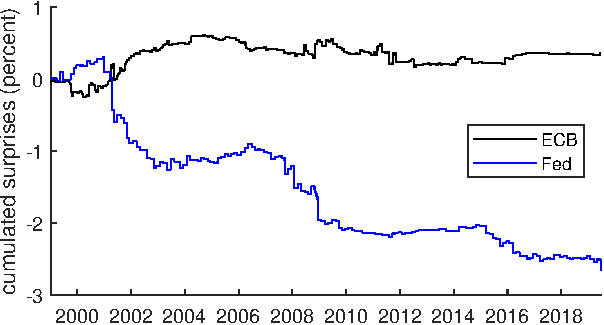
\includegraphics[width=0.47\textwidth]{figures/cumulated_surprises_pc1} &
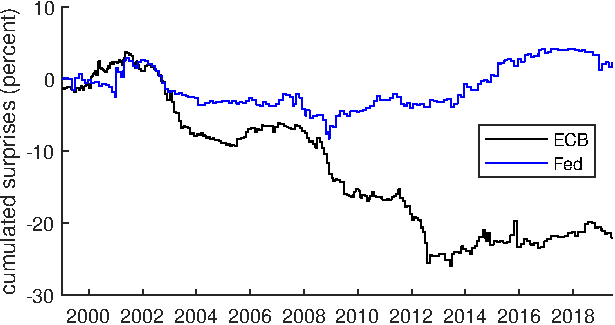
\includegraphics[width=0.47\textwidth]{figures/cumulated_surprises_stock}\\
\end{tabular}
\end{center}
\end{figure}

Table \ref{tab: surprises summary stats} reports the summary statistics of the Fed and ECB
interest rate and stock price surprises.
The ECB interest rate surprises are close to zero on average and have the standard deviation of about 4 basis points. The Fed interest rate surprises are negative on average, -1.55 basis point, and they have a larger standard deviation of 7 basis points. 
Contemporaneous interest rate and stock price surprises are negatively correlated.
For the Fed the correlation is as large as -0.52, suggesting that the monetary policy shocks
dominate, while for the ECB the correlation is only -0.13.
The autocorrelations of the surprises are negligible.
For simplicity I do not further purge these surprises from the component predictable by past information as purging makes little difference for subsequent inference. E.g. \cite{MirandaAgrippino_Ricco_2021} purge the surprises using one of the most comprehensive specifications, by regressing them on
their own lags and ten factors extracted from macroeconomics variables, but the unadjusted R-squared are below 0.1 (see their Table 3).
However, the correlations between the consecutive ECB and Fed surprises have not been explored previously.
Table \ref{tab: surprises correlations} shows that these correlations are small too. The first correlation of -0.13 is significant at the 10\% level but this correlation changes to 0.02
if one omits the large negative Fed surprise on April 18, 2001, which was preceded by a large positive ECB interest rate surprise on April 11.
Low correlations between consecutive shocks guarantee that we don't mistake the effects of domestic policy shocks for transatlantic spillovers.
Figure \ref{fig: cumulated surprises} plots the cumulated surprises of both central banks, interest rate surprises in the left panel and stock price surprises in the right panel. This figure shows that also at lower frequencies there is no systematic correlation between the Fed and ECB surprises.


\subsection{Macroeconomic news surprises}

\begin{itemize}
\item \textbf{Industry confidence} - European Commission Eurozone Industrial Confidence. Ticker: EUICEMU. \emph{Source:} Bloomberg. \emph{Units:} Index.
\item \textbf{Unemployment rate} - Eurostat Unemployment Eurozone SA. Ticker: UMRTEMU. \emph{Source:} Bloomberg. \emph{Units:} Percent.
\end{itemize}


\subsection{Daily financial data}\label{sec: daily data}

\begin{itemize}
\item
\textbf{1-year Bund yield, 10-year Bund yield} - \emph{Source:} Deutsche Bundesbank: Term structure of interest rates on listed Federal securities (method by Svensson) \url{https://www.bundesbank.de/dynamic/action/en/statistics/time-series-databases/time-series-databases/759784/759784?listId=www_skms_it03a}. \emph{Units:} percent. \emph{Transformation:} none.
\item
\textbf{1-year Treasury bond yield, 10-year Treasury bond yield} - Zero-coupon yield, Continuously Compounded. \emph{Source:} 
\url{https://www.federalreserve.gov/pubs/feds/2006/200628/200628abs.html} Identifiers: SVENY01, SVENY10. Reference: 
\cite{Gurkaynak_Sack_Wright_2007} \emph{Units}: percent. \emph{Transformation:} none.
\item
\textbf{S\&P500} - Standard and Poors 500 Composite Index \emph{Source:} Datastream. \emph{Units:} index. \emph{Transformation:} 100*log.
\item
\textbf{Euro Stoxx 50} - Dow Jones Euro Stoxx 50 EUR Price Index - \emph{Source:} Bloomberg. \emph{Units:} index. \emph{Transformation:} 100*log.
\item
\textbf{High yield corporate bond OAS (US)} - ICE BofA US High Yield Index Option-Adjusted Spread (OAS). US dollar denominated below investment grade
rated corporate debt publicly issued in the US domestic market. \emph{Source:} Fred, after Ice Data Indices, LLC. Identifier: bamlh0a0hym2. \emph{Units:} percent. \emph{Transformation:} none.
\item
\textbf{High yield corporate bond OAS (EA)} - ICE BofA Euro High Yield Index Option-Adjusted Spread (OAS). Euro denominated below
investment grade corporate debt publicly issued in the euro domestic  
or eurobond markets. \emph{Source:} Fred, after Ice Data Indices, LLC. Identifier: bamlhe00ehyioas. \emph{Units:} percent. \emph{Transformation:} none.
\item
\textbf{EUR per USD} - Exchange rate. \emph{Source:} ECB. \emph{Units:} Euros per one US dollar. \emph{Transformation:} 100*log.
\item
\textbf{Broad dollar ex EUR} - The Broad dollar index, calculated
by the Federal Reserve, is a trade-weighted exchange rate with respect to 26 most important trading partners by volume of the bilateral trade. I have recalculated this index taking the euro out of it. 
The construction of the Broad dollar index is explained in \cite{Beschwitz_etal_2019},
\url{https://www.federalreserve.gov/econres/notes/feds-notes/revisions-to-the-federal-reserve-dollar-indexes-20190115.htm}. The Broad dollar index back to 2006 was downloaded from the Federal Reserve website \url{https://www.federalreserve.gov/datadownload/Build.aspx?rel=H10}
and the euro's weights back to 2006 was downloaded from \url{https://www.federalreserve.gov/releases/h10/weights/default.htm}. The Broad dollar index and the euro's weights before 2006 were taken from the data appendix of \cite{Beschwitz_etal_2019}, \url{https://www.federalreserve.gov/econres/notes/ifdp-notes/IFDP_Note_Data_Appendix.xlsx}. I have removed the euro from the Broad dollar index and rescaled so that the weights of the remaining currencies add up to 1. 
\emph{Units:} index, foreign currency per one US dollar. \emph{Transformation:} 100*log.

More in detail, the Broad dollar index at time $t$ ($I_t$) is $I_t = I_{t-1} \prod_j^N (e_{j,t}/e_{j,t-1})^{w_{j,t}}$, where $e_{j,t}$ is the price of the dollar in terms of the foreign currency $j$ at time $t$ and $w_{j,t}$ is its weight \citep{Beschwitz_etal_2019}. Let the euro be the $N$th currency, let $\Delta i_t = \ln(I_t/I_{t-1})$ be the log change of the broad dollar index and let $c_{N,t} = w_{N,t}\ln (e_{N,t}/e_{N,t-1})$ be the euro's contribution to it. The log change of the Broad dollar ex EUR is computed as $\Delta i_t^\text{exEUR} = 1/(1-w_{N,t}) (\Delta i_t - c_{N,t})$.
\item
\textbf{S\&P500 Financials} - The S\&P 500 Financials comprises those companies included in the S\&P 500 that are classified as members of the GICS financials sector. Number of companies: 66. Total Return index. Ticker: SPTRFINL.
\emph{Source:} Bloomberg. \emph{Units:} index. \emph{Transformation:} 100*log.
\item
\textbf{S\&P500 Ex-Financials} - The S\&P 500 Ex-Financials is designed to provide broad market exposure except for members of the financials sector.
Number of companies: 439. Total Return index. Ticker: SPXXFIST.
\emph{Source:} Bloomberg. \emph{Units:} index. \emph{Transformation:} 100*log.
\item
\textbf{Wilshire US Small-Cap} - The Wilshire US Small-Cap is a float-adjusted, market capitalization-weighted index of the issues ranked between 750 and 2,500 by market capitalization of the Wilshire 5000 Total Market Index.
 Number of companies: 1745. Fred identifier: WILLSMLCAP.  \emph{Source}: Fred after Wilshire Associates. \emph{Units:} index. \emph{Transformation:} 100*log.
\item
\textbf{Wilshire US Large-Cap} - The Wilshire US Large-Cap Index is a float-adjusted, market capitalization-weighted index of the issues ranked above 750 by market capitalization of the Wilshire 5000 Total Market Index. Together, the components of the Wilshire US Large-Cap, Wilshire US Small-Cap Index and Wilshire US Micro-Cap Index comprise the Wilshire 5000 without gaps or overlaps. Number of companies: 750. Fred identifier: WILLLRGCAP. \emph{Source}: Fred after Wilshire Associates. \emph{Units:} index. \emph{Transformation:} 100*log.
\item
\textbf{Europe-exposed S\&P500, US-exposed S\&P500} - Based on Worldscope and Datastream.
The indices have a fixed composition and consist of 497 stocks that entered the S\&P500 for at least 40 quarters between 1998 and 2020.
For each of those 497 companies I obtain from Worldscope the share of sales in Europe in their total sales in the years 2000, 2005, 2010, 2015, 2020 and average it over time.
I take the daily data on prices and float-adjusted market capitalization from Datastream.
Then I construct a price index of these 497 stocks weighted by the float-adjusted market capitalization multiplied by the shares of European sales.
There are 252 companies with nonzero and non-missing average European sales shares, for 129 companies the share exceeds 10\% and for 90 companies the share exceeds 15\%.
I proceed analogously for the US-exposed companies.
There are 472 companies with nonzero and non-missing average US sales shares, for 175 companies the share exceeds 90\% and for 150 companies the share exceeds 95\%.
\emph{Units:} index. \emph{Transformation:} 100*log.
\item
\textbf{Fed funds futures next FOMC, Fed funds futures 3m, Fed funds futures 6m} - The rates implied by the 30-days federal funds futures after the Next FOMC meeting (based on the current month or next month futures, depending on the date of the next FOMC meeting), in 3-months and in 6-months. \emph{Source}: Haver. Identifiers: PNFP@DAILY, PFFN3P@DAILY and PFFN6P@DAILY \emph{Units:} percent. \emph{Transformation:} none.

\end{itemize}

\subsection{Monthly variables}

\begin{itemize}
\item
\textbf{Effective Federal Funds Rate} - daily average. \emph{Source:} Fred, after Board of Governors of the Federal Reserve System. Identifier: FEDFUNDS. \emph{Units:} Percent. \emph{Transformation:} none.
\item
\textbf{Shadow Federal Funds Rate (Wu-Xia)} - \cite{Wu_Xia_2016}. Downloaded
from \url{https://sites.google.com/view/jingcynthiawu/shadow-rates}.
\emph{Units:} Percent. \emph{Transformation:} none.
\item 
\textbf{Shadow Federal Funds Rate (Krippner)} - \cite{Krippner_2013,Krippner_2015}. Downloaded
from \url{https://www.ljkmfa.com/visitors/}.
\emph{Units:} Percent. \emph{Transformation:} none.
\item
\textbf{Broad euro} - Broad Effective Exchange Rate for Euro Area. \emph{Source:} Fred, after BIS.  Identifier NBXMBIS. \emph{Units:} index, foreign currency per one Euro. \emph{Transformation:} 100*log.
\item
\textbf{US Real GDP and GDP Deflator} - Interpolation by
\cite{Stock_Watson_2010} updated to 2019Q1. See the replication files for \cite{Jarocinski_Karadi_2020}. \emph{Transformation:} 100*log.
\item
\textbf{Euro area Real GDP and GDP Deflator} - Own interpolation following
\cite{Stock_Watson_2010}. See the replication files for \cite{Jarocinski_Karadi_2020}. \emph{Transformation:} 100*log.
\end{itemize}

The remaining monthly variables are the monthly averages of the daily variables discussed in \ref{sec: daily data}.

%%%%%%%%%%%%%%%%%%%%%%%%%%%%%%%%%%%%%%%%%%%%%%%%%%%%%%%%%%%%%%%%%%%%%%%%%%%%%%%%
%%%%%%%%%%%%%%%%%%%%%%%%%%%%%%%%%%%%%%%%%%%%%%%%%%%%%%%%%%%%%%%%%%%%%%%%%%%%%%%%
%%%%%%%%%%%%%%%%%%%%%%%%%%%%%%%%%%%%%%%%%%%%%%%%%%%%%%%%%%%%%%%%%%%%%%%%%%%%%%%%
\subsection{Fed announcement surprises in the press conference windows}\label{sec: Fed press conf}


\paragraph{The dates and times of the Fed press conferences.} 
The dates and times of the Fed post-FOMC meeting press conferences come from the Bloomberg Economic Calendar.
(See also \cite{Bodilsen_etal_2021} for a convenient summary table in their Online Appendix.)
The Fed started to hold press conferences after FOMC meetings on April 27, 2011. 
In the years 2011-2018 the press conferences were held after every other FOMC meeting
and since 2019 after every FOMC meeting.
In the years 2011-2012 the FOMC announcements were published at 12:30 and the press
conferences started at 14:15.
From 2013 onward the FOMC announcement was issued at 14:00 and the press conference started at 14:30.

\paragraph{Press Conference Window} 
I define a Press Conference Window that starts 10 minutes before the start of the press conference
and ends 75 minutes after the start of the press conference.
From 2013 onward the start of the Press Conference Window coincides with the end of the GSS FOMC press release window (the GSS window ends 20 minutes after the press release).
For the 8 press conferences held in the years 2011-2012 there is a gap 
between the end of the GSS window and the start of the Press Conference Window.
The press conferences last approximately one hour, so the Press Conference Window
ends approximately 15 minutes after the end of the press conference,
like in the \cite{Altavilla_etal_2019} dataset of the ECB surprises.


\paragraph{Summary statistics about press conference (PC) surprises.} 
The changes in the PC Window of the variables MP1, FF4, ED2, ED3, ED4 and SP500, defined in \cite{Gurkaynak_Sack_Swanson_2005a} are extracted from the Thomson Reuters Tick History database.
There are 36 press conferences between April 2011 and June 2019.
Figures \ref{fig: fed pr and pc}, \ref{fig: fed pr and pc 2}, \ref{fig: fed pr and pc 3} 
present the GSS surprises for all FOMC announcements from January 1999 until June 2019 along with the PC surprises available for 36 of these FOMC announcements.
Table \ref{tab: fed pr and pc} reports summary statistics computed on these 36 dates.
The PC variance share is defined as var($x^{PC}$)/(var($x^{PC}$)+var($x^{GSS}$)),
where $x^{PC}$ is the surprise in variable $x$ in the PC window and
$x^{GSS}$ is the surprise in variable $x$ in the press release window coming from the GSS database.
The table reports also the correlations between $x^{PC}$ and $x^{GSS}$ and their statistical significance.
First, on the press conference days the press conference windows
account for about one third of the variance of interest rate derivatives with maturities 3 months and more,
and less than that near-term futures MP1. For stock prices the press conference windows
account for 57\% of the variance.
Second, we can see in Figures \ref{fig: fed pr and pc}, \ref{fig: fed pr and pc 2}, \ref{fig: fed pr and pc 3} that in the press conference windows asset prices tend to move
in the same direction as in the preceding announcement windows. 
Indeed, Table \ref{tab: fed pr and pc}
shows that the correlations between the surprises in the two windows are positive, though not always statistically significant.
For the stock prices the correlation is 0.45 and highly significant.


\begin{table}[!htbp]
\begin{center}
\caption{Press conference (PC) surprises - variance shares and correlations with the GSS surprises}\label{tab: fed pr and pc}
\begin{tabular}{p{6cm}ccc}
\toprule
Variable & PC variance share & Corr($x^{PC},x^{GSS}$) & p-value \\
\midrule
MP1 & 0.04 & 0.15 & 0.41 \\
FF4 & 0.29 & 0.19 & 0.28 \\
ED2 & 0.38 & 0.34 & 0.04 \\
ED3 & 0.35 & 0.29 & 0.08 \\
ED4 & 0.29 & 0.23 & 0.17 \\
Total $i$ surprise (i.e. the 1st Principal Component of the above) & 0.31 & 0.29 & 0.09 \\
SP500 & 0.57 & 0.45 & 0.01 \\
\bottomrule
\end{tabular}
\end{center}\footnotesize
Note. The PC variance share of variable $x$ is defined as var($x^{PC}$)/(var($x^{PC}$)+var($x^{GSS}$)).
The p-value indicates the statistical significance of the correlation.
Both the variance shares and the correlations are computed over the 36 observations
with press conferences.
\end{table}


\renewcommand{\pathA}{../data/shocks/plots_pconf}
\begin{figure}[p]
\caption{Fed surprises in the Press Release and Press Conference windows}\label{fig: fed pr and pc}
\begin{center}
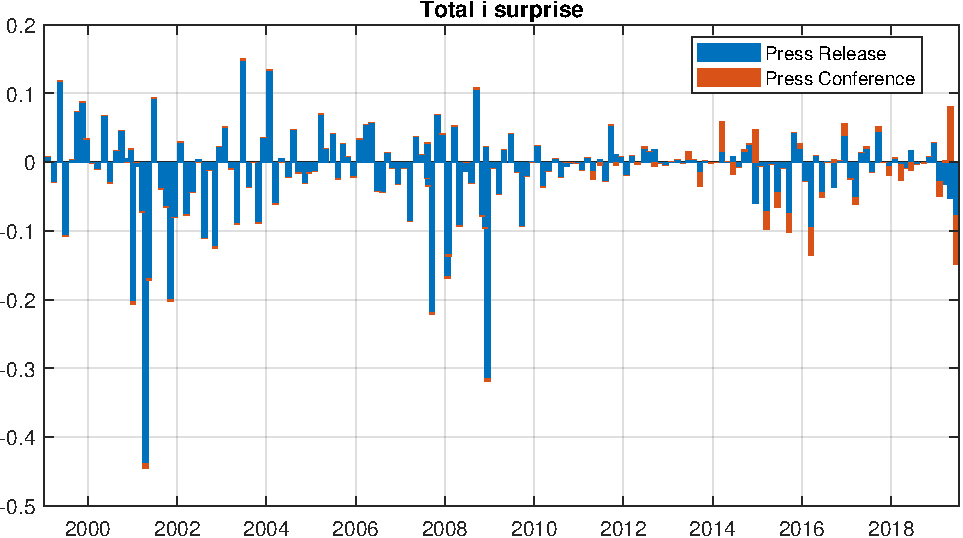
\includegraphics[width=0.7\textwidth]{\pathA/contrib_pr_pc_pc1ff1_pr}\\
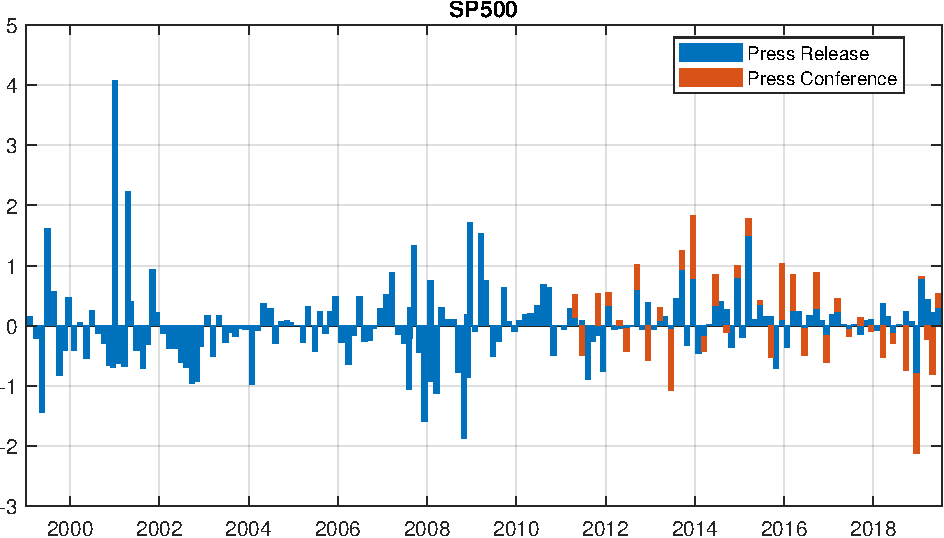
\includegraphics[width=0.7\textwidth]{\pathA/contrib_pr_pc_SP500}\\
\end{center}
\footnotesize Note. Blue bars show the surprises in the press release window, from GSS. Red bars show the surprises in the press conference window, from Thomson Reuters Tick History.
\end{figure}

\begin{figure}[p]
\caption{Fed surprises in the Press Release and Press Conference windows - continued}\label{fig: fed pr and pc 2}
\begin{center}
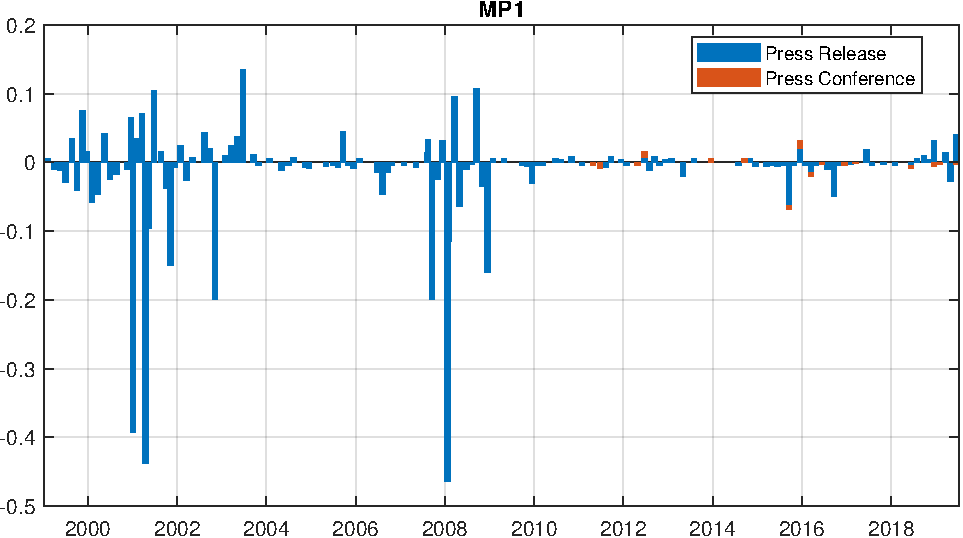
\includegraphics[width=0.7\textwidth]{\pathA/contrib_pr_pc_MP1}\\
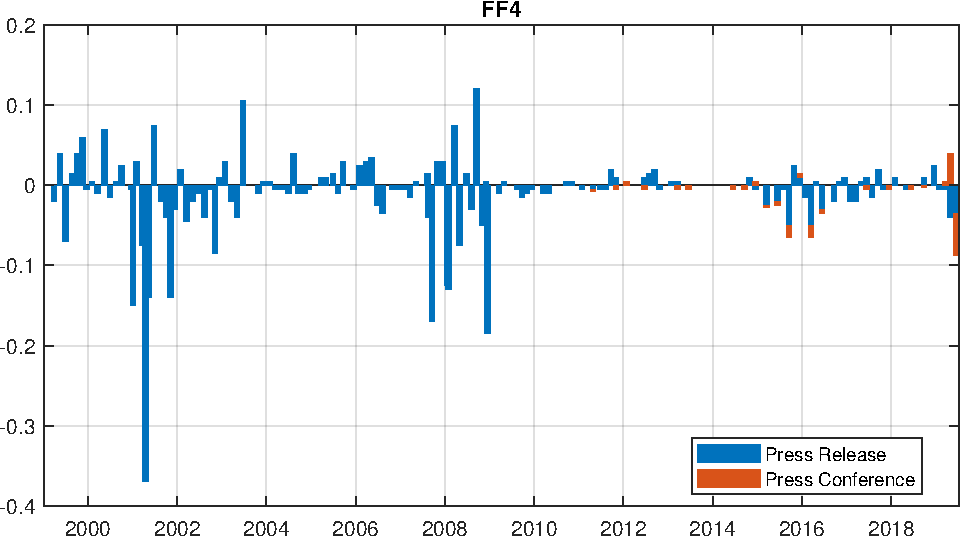
\includegraphics[width=0.7\textwidth]{\pathA/contrib_pr_pc_FF4}\\
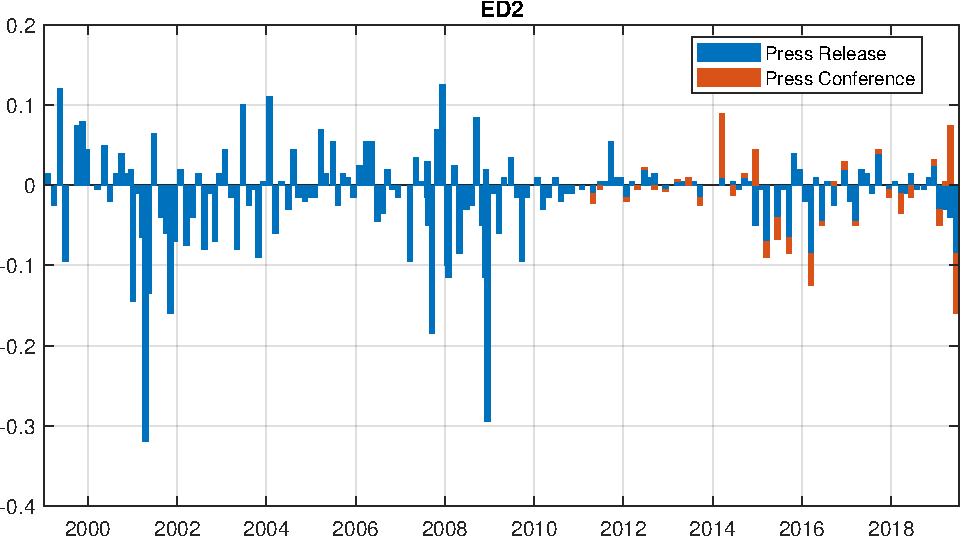
\includegraphics[width=0.7\textwidth]{\pathA/contrib_pr_pc_ED2}\\
\end{center}
\footnotesize Note. Blue bars show the surprises in the press release window, from GSS. Red bars show the surprises in the press conference window, from Thomson Reuters Tick History.
\end{figure}

\begin{figure}[p]
\caption{Fed surprises in the Press Release and Press Conference windows - continued}\label{fig: fed pr and pc 3}
\begin{center}
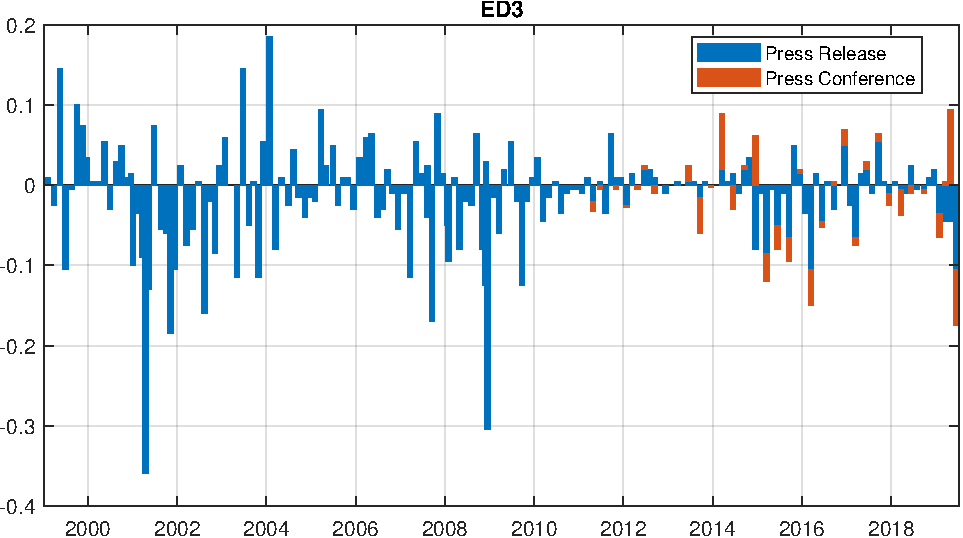
\includegraphics[width=0.7\textwidth]{\pathA/contrib_pr_pc_ED3}\\
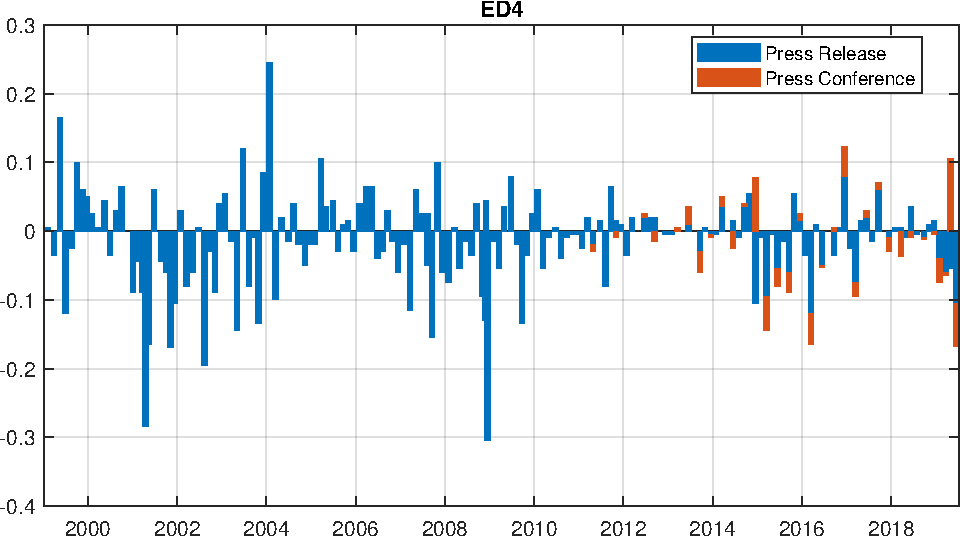
\includegraphics[width=0.7\textwidth]{\pathA/contrib_pr_pc_ED4}\\
\end{center}
\footnotesize Note. Blue bars show the surprises in the press release window, from GSS. Red bars show the surprises in the press conference window, from Thomson Reuters Tick History.
\end{figure}


\clearpage

%%%%%%%%%%%%%%%%%%%%%%%%%%%%%%%%%%%%%%%%%%%%%%%%%%%%%%%%%%%%%%%%%%%%%%%%%%%%%%%%
%%%%%%%%%%%%%%%%%%%%%%%%%%%%%%%%%%%%%%%%%%%%%%%%%%%%%%%%%%%%%%%%%%%%%%%%%%%%%%%%
%%%%%%%%%%%%%%%%%%%%%%%%%%%%%%%%%%%%%%%%%%%%%%%%%%%%%%%%%%%%%%%%%%%%%%%%%%%%%%%%
\section{Rotational sign restrictions}
This section explains the details of rotational sign restrictions. Recall that the goal is to decompose the interest rate surprises into a sum of two orthogonal
components, such that the first one is associated with a negative
co-movement of the interest rate and stock price surprises and the second is associated with their positive co-movement.

Recall also that $i^{Total}$ is a vector of interest rate surprises, $s$ is a vector of stock price surprises, $i^{MP}$ is a vector of monetary policy shock proxies and $i^{CBI}$ is a vector of central bank information shock proxies. Each of the four vectors has length $T$, where $T$ is the number of central bank announcements in the dataset. Let $M=(i^{Total},s)$ be a $T \times 2$ matrix with columns $i^{Total}$ and $s$.
I decompose $M$ as
\begin{equation} M = UC,\quad  \text{where}\quad U=\left(i^{MP},i^{CBI}\right), \quad (i^{MP})'i^{CBI}=0 \quad \text{and}\quad
C=\begin{pmatrix}1&c_{MP}<0\\1&c_{CBI}>0\end{pmatrix}.\label{eq: rotational sign restrictions}
\end{equation}

The decomposition in (\ref{eq: rotational sign restrictions}) is not unique. There is a range of ``rotations'' of $U$ and $C$ that all satisfy the sign restrictions $c_{MP}<0$ and $c_{CBI}>0$. 

\subsection{Computing the decomposition}
$U$ and $C$ are computed as
\begin{equation}
U = QPD \quad \text{and} \quad C = D^{-1}P'R
\end{equation}
where the matrices $Q,P,D,R$ are obtained in three steps.

\bigskip
\noindent 1. \emph{Decompose $M$ into two orthogonal components} using the QR decomposition,
\begin{equation}
M = QR,\quad  \text{where}\quad Q'Q=\begin{pmatrix}1&0\\0&1\end{pmatrix}\quad \text{and}\quad
R=\begin{pmatrix}r_{11}>0&r_{12}\\0&r_{22}>0\end{pmatrix}.
\end{equation}
Note that in many software packages do not impose the normalization that the diagonal elements of $R$ are positive, in this case this has to be imposed ex post.

\bigskip
\noindent 2. \emph{Rotate} these orthogonal components using the rotation matrix $P$,
\begin{equation} P = \begin{pmatrix}\cos(\alpha)&\sin(\alpha)\\-\sin(\alpha)&\cos(\alpha)\end{pmatrix}.
\end{equation}
- To satisfy the sign restrictions use any angle $\alpha$ in the following range
\begin{subequations}
\begin{align}
\alpha\in\left(0,\arctan\frac{-r_{22}}{r_{12}}\right)\quad\text{if}\quad&r_{12}<0,\label{eq: angle range rhoneg}\\
\alpha\in\left(\arctan\frac{r_{12}}{r_{22}},\frac{\pi}{2}\right)\quad\text{if}\quad&r_{12}\ge0.\label{eq: angle range rhopos}
\end{align}
\end{subequations}
- To obtain the desired variance share $\operatorname{var}(i^{MP})/\operatorname{var}(i^{Total})$ use
\begin{equation}
\alpha = \arccos \sqrt{\frac{\operatorname{var}(i^{MP})}{\operatorname{var}(i^{Total})}}.
\end{equation}

\bigskip
\noindent 3.  \emph{Rescale} the resulting orthogonal components with a diagonal matrix $D$ to ensure that they add up to the interest rate surprises $i^{Total}$. It is straightforward to show that
\begin{equation} D = \begin{pmatrix}r_{11} \cos(\alpha)&0\\0&r_{11}\sin(\alpha)\end{pmatrix}.\label{eq: D}\end{equation}

\subsection{Properties and derivations}

\emph{Result 1.} The variance shares implied by the above decomposition are
\begin{equation}
\frac{\operatorname{var}(i^{MP})}{\operatorname{var}(i^{Total})}=\cos^2(\alpha) \quad \text{and} \quad
\frac{\operatorname{var}(i^{CBI})}{\operatorname{var}(i^{Total})}=\sin^2(\alpha).\label{eq: varshares and angle}
\end{equation}

\emph{Proof} This is the straightforward implication of using the matrix $D$ given in (\ref{eq: D}) in $U=QPD$.$\blacksquare$

\noindent\emph{Result 2.} Considering $\alpha\in(-\pi,\pi)$, the sign restrictions $c_{MP}<0$ and $c_{CBI}>0$ are satisfied if and only if $\alpha$ satisfies (\ref{eq: angle range rhoneg})-(\ref{eq: angle range rhopos}).

\emph{Proof.}
Consider the ``unscaled'' decomposition $M=\tilde{U}\tilde{C}$ where $\tilde{U}=QP$ and $\tilde{C}=P'R$. $\tilde{C}$  contains the impact of the two ``unscaled'' shocks in $\tilde{U}$ on the interest rate and stock price surprises, so $\tilde{C}$ should satisfy
\[ \tilde{C}=\begin{pmatrix}\tilde{c}_{11}>0&\tilde{c}_{12}<0\\\tilde{c}_{21}>0&\tilde{c}_{22}>0\end{pmatrix}\]
$\tilde{C}=P'R$ implies the following system of inequalities
\begin{align}
r_{11}\cos\alpha &>0 \label{eq: sys1}\\
r_{12} \cos\alpha -r_{22}\sin\alpha &<0\label{eq: sys2}\\
r_{11}\sin\alpha&>0\label{eq: sys3}\\
r_{12} \sin\alpha+r_{22}\cos\alpha&>0\label{eq: sys4}
\end{align}
Assume without loss of generality that $\alpha\in(-\pi,\pi)$.  (\ref{eq: sys1}) and (\ref{eq: sys3}) imply that $\alpha\in(0,\pi/2)$.
If $r_{12}<0$, (\ref{eq: sys2}) is slack and (\ref{eq: sys4}) implies (\ref{eq: angle range rhoneg}).
If $r_{12}>0$, (\ref{eq: sys4}) is slack and (\ref{eq: sys2}) implies (\ref{eq: angle range rhopos}).
$\blacksquare$

\noindent\emph{Result 3.} The variance share of the monetary policy shock must be within the following bounds:
\begin{equation}
\frac{\operatorname{var}(i^{MP})}{\operatorname{var}(i^{Total})} \in 
\begin{cases}
(\rho^2,1) & \text{if } \rho<0, \\
(0,1-\rho^2) & \text{if } \rho\ge 0.
\end{cases}\label{eq: ranges varshare1}
\end{equation}

\emph{Proof.}
This follows from (\ref{eq: angle range rhoneg}), (\ref{eq: angle range rhopos}) and (\ref{eq: varshares and angle}).
To simplify the expressions use the fact that $\cos(\arctan(x))=1/\sqrt{1+x^2}$. This implies
\begin{equation}
\frac{\operatorname{var}(i^{MP})}{\operatorname{var}(i^{Total})}\in
\left(\frac{r_{12}^2}{r_{22}^2+r_{12}^2},1\right) \text{if }  r_{12}<0 \text{ and }
\frac{\operatorname{var}(i^{MP})}{\operatorname{var}(i^{Total})}
\in\left(0,\frac{r_{22}^2}{r_{12}^2+r_{22}^2}\right) \text{if }  r_{12}\ge0.
\end{equation}
To simplify further notice that $M'M=R'Q'QR=R'R$, and hence
\begin{equation}
\begin{pmatrix}i^{Total\prime}i^{Total} & i^{Total\prime}s\\ \dots & s's \end{pmatrix}=
\begin{pmatrix}r_{11}^2 & r_{11}r_{12}\\ \dots & r_{12}^2+r_{22} ^2\end{pmatrix}.\blacksquare
\end{equation}

\subsection{Results for the Fed and ECB surprises studied in this paper}

\begin{figure}[!htbp]
\caption{Alternative sign restriction-based decompositions of central bank surprises.}\label{fig: rotation extremes}
\begin{center}
\begin{tabular}{cc}
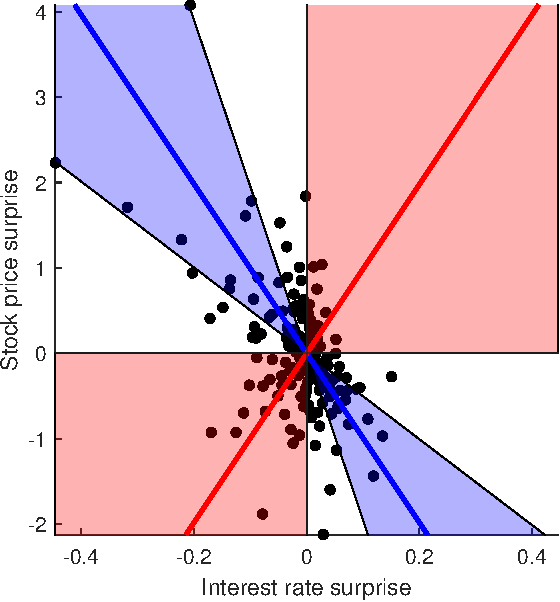
\includegraphics[width=0.45\textwidth]{figures/fed-scatter-rotations}&
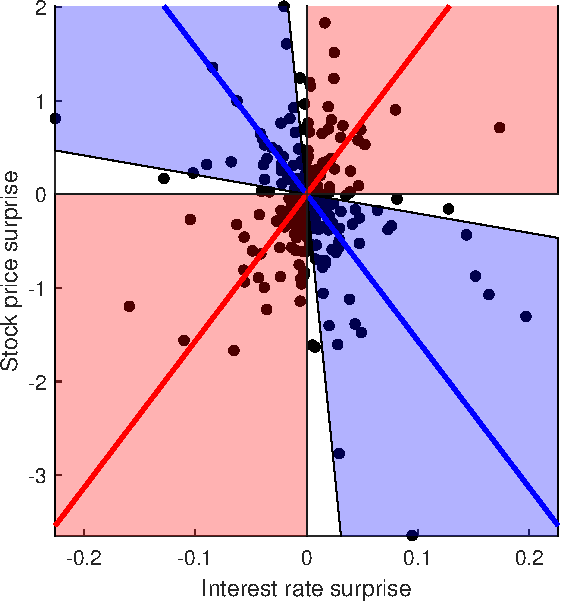
\includegraphics[width=0.45\textwidth]{figures/ecb-scatter-rotations}\\
Fed announcements & ECB announcements
\end{tabular}
\end{center}
\footnotesize Note. Each dot corresponds to one announcement. In each plot, the blue line represents the relationship $s = c_{MP}* i^{MP}$ and the red line represents the relationship 
$s = c_{CBI}* i^{CBI}$ for the median rotation. Blue and red ranges represent the slopes of these relations for all the admissible decompositions.
\end{figure}

Figure \ref{fig: rotation extremes} reports the surprises and the admissible range of decompositions.
The scatter plots show the interest rate surprises and stock price
surprises for all Fed and ECB announcements.
The blue regions indicate all the admissible negative relations between $i^{Total}$ and $s$ conditionally on
the monetary policy shock, i.e. all the admissible lines  $s = c_{MP}\,i^{MP}$. 
The red regions indicate all the corresponding positive relations between $i^{Total}$ and $s$ conditionally on
the central bank shock, i.e. all the admissible lines  $s = c_{CBI}\,i^{CBI}$. 

\begin{table}[!htbp]
\begin{center}
\caption{Coefficients $c_{MP}$ and $c_{CBI}$ and variance shares corresponding to selected rotations}\label{tab: rotations}
\begin{tabular}{lccccccc}
\toprule
Percentile of the   & \multicolumn{3}{c}{Fed} & & \multicolumn{3}{c}{ECB}  \\
admissible rotations & $c_{MP}$ & $c_{CBI}$ & $\vsmp$ & & $c_{MP}$ & $c_{CBI}$ & $\vsmp$\\
\midrule
00th & -5.0 & $\infty$ & 1.00 &   & -2.1 & $\infty$ & 1.00 \\
25th & -7.3 & 27.1 & 0.93 &   & -7.9 & 39.3 & 0.88 \\
50th & -9.9 & 9.9 & 0.75 &   &-15.7 & 15.7 & 0.57 \\
75th & -13.5 & 3.6 & 0.51 &   &-31.1 & 6.3 & 0.22 \\
100th & -19.5 & 0.0 & 0.26 &   & -118.8 & 0.0 & 0.02 \\
\bottomrule
\end{tabular}
\end{center}
\end{table}

Table \ref{tab: rotations} reports the coefficients $c_{MP},c_{CBI}$ and variance shares $\vsmp$ for selected rotations. 
Smaller rotation angles produce $i^{MP}$ shocks that affect stock price surprises less and account for a higher share of variance of $i^{Total}$.
For both the ECB and the Fed the smallest admissible rotation angle corresponds to the recursive decomposition and implies that all interest rate surprises are interpreted as monetary policy shocks $i^{MP}$ (and the unexplained variation in stock price surprises is attributed to the `FOMC risk shock' as in \citealt{Kroencke_etal_2021}).

\section{Local projection results}

\subsection{Additional local projection results}

\renewcommand\textfraction{.02}
%%%%%%%%%%%%%%%%%%%%%%%%%% ECB surprises

\begin{table}[!htbp]
\begin{center}
\caption{The effect of ECB interest rate surprises and shocks on financial variables}\label{tab: reg ecb surp}
$y^{}_{t+h}-y^{}_{t-1} = \alpha + \beta_h\, i^{Total,ECB}_t + u_t.$\\
$y^{}_{t+h}-y^{}_{t-1} = \alpha + \beta^{MP}_h\, i^{MP}_t + \beta^{CBI}_h\, i^{CBI}_t + u_t.$
\small
\resizebox{0.95\textwidth}{!}{
\begin{tabular}{lcccccccccc} \toprule
 & $h=1$ & $h=2$ & $h=3$ & $h=4$ & $h=5$ & $h=10$ & $h=15$ & $h=20$ & $h=25$ & $h=30$
\input{\pathTables table-ecbsurp1a.txt}\\[-0.9cm]
\input{\pathTables table-ecbsurp1b.txt}
\tabularnewline\bottomrule
\end{tabular}}
\end{center}\footnotesize
Notes: Heteroskedasticity robust standard errors in parentheses. *** p$<$0.01, ** p$<$0.05, * p$<$0.1.
Constant terms are not reported for brevity.
\end{table}

%%%%%%%%%%%%%%%%%%%%%%%%%% ECB shocks: Fed funds futures


\begin{table}[!htbp]\small
\begin{center}
\caption{The effect of ECB monetary policy and information shocks on Fed funds futures, omitting the Zero Lower Bound period.}\label{tab: lp ecb shocks fff nozlb}
\resizebox{\textwidth}{!}{
\begin{tabular}{lcccccccccc} \toprule
 & $h=1$ & $h=2$ & $h=3$ & $h=4$ & $h=5$ & $h=10$ & $h=15$ & $h=20$ & $h=25$ & $h=30$
\input{\pathTables table-ecbshocks4.txt}
\tabularnewline\bottomrule
\end{tabular}
}
\end{center}
Notes: Heteroskedasticity robust standard errors in parentheses. *** p$<$0.01, ** p$<$0.05, * p$<$0.1.
Constant terms are not reported for brevity.
Ftest: p-value of the F-test for H0: $\beta^{MP}_h=\beta^{CBI}_h$.
The sample excludes the period between 16 December 2008 and 15 December 2015, when the Fed funds rate was stuck near zero.
\end{table}

\clearpage

\subsection{Local projection results corresponding to the figures in the text}

%%%%%%%%%%%%%%%%%%%%%%%%%% ECB shocks
\begin{table}[!htbp]
\begin{center}
\caption{The effect of ECB monetary policy and information shocks on financial variables}\label{tab: lp ecb shocks}
$y^{}_{t+h}-y^{}_{t-1} = \alpha + \beta^{MP}_h\, i^{MP}_t + \beta^{CBI}_h\, i^{CBI}_t + u_t.$
\small
\resizebox{\textwidth}{!}{
\begin{tabular}{lcccccccccc} \toprule
 & $h=1$ & $h=2$ & $h=3$ & $h=4$ & $h=5$ & $h=10$ & $h=15$ & $h=20$ & $h=25$ & $h=30$
\input{\pathTables table-ecbshocks2.txt}
\tabularnewline\bottomrule
\end{tabular}}
\end{center}\footnotesize
Notes: Heteroskedasticity robust standard errors in parentheses. *** p$<$0.01, ** p$<$0.05, * p$<$0.1.
Constant terms are not reported for brevity.
Ftest: p-value of the F-test for H0: $\beta^{MP}_h=\beta^{CBI}_h$.
\end{table}


\begin{table}[!htbp]\addtocounter{table}{-1}\small
\begin{center}
\caption{Continued}
\resizebox{\textwidth}{!}{
\begin{tabular}{lcccccccccc} \toprule
 & $h=1$ & $h=2$ & $h=3$ & $h=4$ & $h=5$ & $h=10$ & $h=15$ & $h=20$ & $h=25$ & $h=30$
\input{\pathTables table-ecbshocks3.txt}
\tabularnewline\bottomrule
\end{tabular}}
\end{center}\footnotesize
Notes: Heteroskedasticity robust standard errors in parentheses. *** p$<$0.01, ** p$<$0.05, * p$<$0.1.
Constant terms are not reported for brevity.
Ftest: p-value of the F-test for H0: $\beta^{MP}_h=\beta^{CBI}_h$.
\end{table}


%%%%%%%%%%%%%%%%%%%%%%%%%% EA macro surprises

\begin{table}[!htbp]
\begin{center}
\caption{The effect of European industrial confidence surprises on financial variables}\label{tab: lp z ea bcs confind}
$y^{}_{t+h}-y^{}_{t-1} = \alpha + \beta_h\, z^{IndConf}_t + u_t$
\small
\resizebox{0.97\textwidth}{!}{
\begin{tabular}{lcccccccccc} \toprule
 & $h=1$ & $h=2$ & $h=3$ & $h=4$ & $h=5$ & $h=10$ & $h=15$ & $h=20$ & $h=25$ & $h=30$
\input{\pathTables table-z_ea_bcs_confind.txt}
\tabularnewline\bottomrule
\end{tabular}}
\end{center}\footnotesize
Notes: Heteroskedasticity robust standard errors in parentheses. *** p$<$0.01, ** p$<$0.05, * p$<$0.1.
Constant terms are not reported for brevity.
\end{table}

\begin{table}[!htbp]
\begin{center}
\caption{The effect of euro area unemployment rate surprises on financial variables}\label{tab: lp z ea unemp}
$y^{}_{t+h}-y^{}_{t-1} = \alpha + \beta_h\, z^{Unemp}_t + u_t$
\small
\resizebox{0.97\textwidth}{!}{
\begin{tabular}{lcccccccccc} \toprule
 & $h=1$ & $h=2$ & $h=3$ & $h=4$ & $h=5$ & $h=10$ & $h=15$ & $h=20$ & $h=25$ & $h=30$
\input{\pathTables table-z_ea_unemp.txt}
\tabularnewline\bottomrule
\end{tabular}}
\end{center}\footnotesize
Notes: Heteroskedasticity robust standard errors in parentheses. *** p$<$0.01, ** p$<$0.05, * p$<$0.1.
Constant terms are not reported for brevity.
\end{table}

%%%%%%%%%%%%%%%%%%%%%%%%%% ECB shocks: Stocks

\begin{table}[!htbp]\small
\begin{center}
\caption{The effect of ECB monetary policy and information shocks on stock sub-indices.}\label{tab: lp ecb shocks stocks}
\resizebox{\textwidth}{!}{
\begin{tabular}{lcccccccccc} \toprule
 & $h=1$ & $h=2$ & $h=3$ & $h=4$ & $h=5$ & $h=10$ & $h=15$ & $h=20$ & $h=25$ & $h=30$
\input{\pathTables table-ecbshocks-stocks1.txt}
\tabularnewline\bottomrule
\end{tabular}
}
\end{center}
Notes: Heteroskedasticity robust standard errors in parentheses. *** p$<$0.01, ** p$<$0.05, * p$<$0.1.
Constant terms are not reported for brevity.
Ftest: p-value of the F-test for H0: $\beta^{MP}_h=\beta^{CBI}_h$.
\end{table}

\begin{table}[!htbp]\addtocounter{table}{-1}\small
\begin{center}
\caption{Continued}
\resizebox{\textwidth}{!}{
\begin{tabular}{lcccccccccc} \toprule
 & $h=1$ & $h=2$ & $h=3$ & $h=4$ & $h=5$ & $h=10$ & $h=15$ & $h=20$ & $h=25$ & $h=30$
\input{\pathTables table-ecbshocks-stocks2.txt}
\tabularnewline\bottomrule
\end{tabular}}
\end{center}
Notes: Heteroskedasticity robust standard errors in parentheses. *** p$<$0.01, ** p$<$0.05, * p$<$0.1.
Constant terms are not reported for brevity.
Ftest: p-value of the F-test for H0: $\beta^{MP}_h=\beta^{CBI}_h$.
\end{table}

\begin{table}[!htbp]\addtocounter{table}{-1}\small
\begin{center}
\caption{Continued}
\resizebox{\textwidth}{!}{
\begin{tabular}{lcccccccccc} \toprule
 & $h=1$ & $h=2$ & $h=3$ & $h=4$ & $h=5$ & $h=10$ & $h=15$ & $h=20$ & $h=25$ & $h=30$
\input{\pathTables table-ecbshocks-stocks3.txt}
\tabularnewline\bottomrule
\end{tabular}}
\end{center}
Notes: Heteroskedasticity robust standard errors in parentheses. *** p$<$0.01, ** p$<$0.05, * p$<$0.1.
Constant terms are not reported for brevity.
Ftest: p-value of the F-test for H0: $\beta^{MP}_h=\beta^{CBI}_h$.
\end{table}

%%%%%%%%%%%%%%%%%%%%%%%%%% EA macro surprises - stocks

\begin{table}[!htbp]
\begin{center}
\caption{The effect of European industrial confidence surprises on stock sub-indices}\label{tab: lp z ea bcs confind stocks}
$y^{}_{t+h}-y^{}_{t-1} = \alpha + \beta_h\, z^{IndConf}_t + u_t$
\small
\resizebox{0.97\textwidth}{!}{
\begin{tabular}{lcccccccccc} \toprule
 & $h=1$ & $h=2$ & $h=3$ & $h=4$ & $h=5$ & $h=10$ & $h=15$ & $h=20$ & $h=25$ & $h=30$
\input{\pathTables table-z_ea_bcs_confind-stocks.txt}
\tabularnewline\bottomrule
\end{tabular}}
\end{center}\footnotesize
Notes: Heteroskedasticity robust standard errors in parentheses. *** p$<$0.01, ** p$<$0.05, * p$<$0.1.
Constant terms are not reported for brevity.
\end{table}

\begin{table}[!htbp]
\begin{center}
\caption{The effect of euro area unemployment rate surprises on stock sub-indices}\label{tab: lp z ea unemp stocks}
$y^{}_{t+h}-y^{}_{t-1} = \alpha + \beta_h\, z^{Unemp}_t + u_t$
\small
\resizebox{0.97\textwidth}{!}{
\begin{tabular}{lcccccccccc} \toprule
 & $h=1$ & $h=2$ & $h=3$ & $h=4$ & $h=5$ & $h=10$ & $h=15$ & $h=20$ & $h=25$ & $h=30$
\input{\pathTables table-z_ea_unemp-stocks.txt}
\tabularnewline\bottomrule
\end{tabular}}
\end{center}\footnotesize
Notes: Heteroskedasticity robust standard errors in parentheses. *** p$<$0.01, ** p$<$0.05, * p$<$0.1.
Constant terms are not reported for brevity.
\end{table}


%%%%%%%%%%%%%%%%%%%%%%%%%% Fed shocks

\begin{table}[!htbp]
\begin{center}
\caption{The effect of Fed monetary policy and information shocks on financial variables}\label{tab: reg fed shocks}
$y^{}_{t+h}-y^{}_{t-1} = \alpha + \beta^{MP}_h\, i^{MP}_t + \beta^{CBI}_h\, i^{CBI}_t + u_t.$
\small
\resizebox{\textwidth}{!}{
\begin{tabular}{lcccccccccc} \toprule
 & $h=1$ & $h=2$ & $h=3$ & $h=4$ & $h=5$ & $h=10$ & $h=15$ & $h=20$ & $h=25$ & $h=30$
\input{\pathTables table-fedshocks1.txt}
\tabularnewline\bottomrule
\end{tabular}}
\end{center}\footnotesize
Notes: Heteroskedasticity robust standard errors in parentheses. *** p$<$0.01, ** p$<$0.05, * p$<$0.1.
Constant terms are not reported for brevity.
Ftest: p-value of the F-test for H0: $\beta^{MP}_h=\beta^{CBI}_h$.
\end{table}

\begin{table}[!htbp]\addtocounter{table}{-1}\small
\begin{center}
\caption{Continued}
\resizebox{\textwidth}{!}{
\begin{tabular}{lcccccccccc} \toprule
 & $h=1$ & $h=2$ & $h=3$ & $h=4$ & $h=5$ & $h=10$ & $h=15$ & $h=20$ & $h=25$ & $h=30$
\input{\pathTables table-fedshocks2.txt}
\tabularnewline\bottomrule
\end{tabular}}
\end{center}\footnotesize
Notes: Heteroskedasticity robust standard errors in parentheses. *** p$<$0.01, ** p$<$0.05, * p$<$0.1.
Constant terms are not reported for brevity.
Ftest: p-value of the F-test for H0: $\beta^{MP}_h=\beta^{CBI}_h$.
\end{table}


\clearpage

\section{Additional VAR results}\label{sec: app var}

\subsection{Simple (``poor man'') decomposition}

\begin{figure}[!htbp]
\caption{The effects of ECB shocks on the US variables: Impulse responses to one standard deviation  MP and CBI shocks obtained with the simple decomposition in monthly VARs.}\label{fig: var ecb shocks poorman}
\renewcommand{\pathFigures}{../workm_var/ecb/us_gdp_ecb_pm}
\newcommand{\myfig}[1]{\includegraphics[width=0.37\textwidth]{\pathFigures-#1}}
\begin{center}
\begin{tabular}{cc}
\myfig{sveny01_a}&
\myfig{sveny10_a}\\
\myfig{sp500_a}&
\myfig{bofaml_us_hyld_oas_a}\\
\myfig{eurusd_a}&
\myfig{broadexea_usd_a}\\
\myfig{us_rgdp}&
\myfig{us_gdpdef}\\
\end{tabular}
\end{center}
\footnotesize Note: The red solid-dotted lines represent the point-wise posterior medians of the impulse responses to the central bank information shock. The red areas show pointwise 16-84 percentile bands. 
The blue solid lines and blue areas show the same objects for the monetary policy shock. 
The figure is based on 10,000 draws from the Gibbs sampler.
\end{figure}

\subsection{Domestic effects of monetary policies}

\begin{figure}[!htbp]
\caption{The effects of ECB shocks on the euro area variables: Impulse responses to one standard deviation ``rotation-based''  MP and CBI shocks in monthly VARs.}\label{fig: var ecb shocks rotation domestic}
\renewcommand{\pathFigures}{../workm_var/ecb/ea_gdp_ecb_sgnm2}
\newcommand{\myfig}[1]{\includegraphics[width=0.35\textwidth]{\pathFigures-#1}}
\newcommand{\myfigx}[1]{\includegraphics[width=0.35\textwidth]{../workm_var/ecb/#1}}
\begin{center}
\begin{tabular}{cc}
\myfigx{ea_wx_ecb_sgnm2-ea_wuxia} & \myfigx{ea_kr_ecb_sgnm2-ea_krippner}\\
\myfig{bund1y_a} & \myfig{bund10y_a}\\
\myfig{stoxx50_a} & \myfig{bofaml_ea_hyld_oas_a}\\
\myfig{eurusd_a} & \myfig{broad_eur}\\
\myfig{ea_rgdp} & \myfig{ea_gdpdef}\\
\end{tabular}
\end{center}
\footnotesize Note: The red solid-dotted lines represent the point-wise posterior medians of the impulse responses to the central bank information shock. The red areas show pointwise 16-84 percentile bands. 
The blue solid lines and blue areas show the same objects for the monetary policy shock. 
The figure is based on 10,000 draws from the Gibbs sampler.
\end{figure}

\begin{figure}[!htbp]
\caption{The effects of Fed shocks on the US variables: Impulse responses to one standard deviation ``rotation-based''  MP and CBI shocks in monthly VARs.}\label{fig: var fed shocks rotation domestic}
\renewcommand{\pathFigures}{../workm_var/fed/us_gdp_fed_sgnm2}
\newcommand{\myfig}[1]{\includegraphics[width=0.35\textwidth]{\pathFigures-#1}}
\newcommand{\myfigx}[1]{\includegraphics[width=0.35\textwidth]{../workm_var/fed/#1}}
\begin{center}
\begin{tabular}{cc}
\myfigx{us_wx_fed_sgnm2-us_wuxia} & \myfigx{us_kr_fed_sgnm2-us_krippner}\\
\myfig{sveny01_a} & \myfig{sveny10_a}\\
\myfig{sp500_a} & \myfig{bofaml_us_hyld_oas_a}\\
\myfig{eurusd_a} & \myfig{broadexea_usd_a}\\
\myfig{us_rgdp} & \myfig{us_gdpdef}\\
\end{tabular}
\end{center}
\footnotesize Note: The red solid-dotted lines represent the point-wise posterior medians of the impulse responses to the central bank information shock. The red areas show pointwise 16-84 percentile bands. 
The blue solid lines and blue areas show the same objects for the monetary policy shock. 
The figure is based on 10,000 draws from the Gibbs sampler.
\end{figure}

\clearpage
\bibliographystyle{econ}
\bibliography{spillovers}

\end{document}
